\documentclass[11pt,oneside]{uhthesis}
\usepackage{subfigure}
\usepackage[linesnumbered,lined,titlenumbered,ruled]{algorithm2e}
\usepackage{amsmath}
\usepackage{amssymb}
\usepackage{amsbsy}
\usepackage{mathpazo}
\usepackage{float}
\usepackage{braket}
%\usepackage{subcaption}
\setlength {\marginparwidth }{3cm}
\usepackage{todonotes}
% \usepackage{refcheck}
\usepackage{listings}
\usepackage{color}
\usepackage{booktabs}
\usepackage{multirow}
\usepackage{ragged2e}

%\floatstyle{ruled}
%\restylefloat{table}

\renewcommand{\tablename}{Tabla}
%\usepackage{syntax}
%\dontprintsemicolon
\title{Una propuesta para la codificación de soluciones del Problema de Enrutamiento de Vehículos a un espacio continuo}
\author{Dalianys Pérez Perera}
\advisor{MSc. Fernando Rodríguez Flores}
\coadvisor{	Lic. Alain Cartaya Salabarría}
\degree{Licenciado en Ciencias de la Computación}
\faculty{Facultad de Matemática y Computación}
\date{Noviembre de 2021}
\logo{Graphics/uhlogo}
%\makenomenclature

\renewcommand{\vec}[1]{\boldsymbol{#1}}
\newcommand{\diff}[1]{\ensuremath{\mathrm{d}#1}}

\begin{document}
\selectlanguage{spanish}

\frontmatter
\maketitle

\begin{dedication}
	\textit{
		A mis padres,\\ 
		a mi hermano,\\
		a Alain, \\
		a Sinaile,\\
		a mi familia,\\
		a todos los que confiaron en mí cuando yo no creía.}
\end{dedication}
\chapter*{Agradecimientos}\label{chapter:agradecimientos}

Un agradecimiento especial a mis padres, por estar siempre presentes en mi vida, por apoyarme y consentirme en todo momento.\\

A mi tía Marilín por acogerme como otra hija más durante esta etapa. \\

A Alain por ser el mejor maestro, ejemplo y compañero de viaje.\\

A Dayany Alfaro González por brindarme su amistad y las largas horas de estudio. \\

A Ashley Tejeda Meneses por siempre estar en los buenos y malos momentos. \\

A la familia cojimera, muchas gracias por abrirme sus puertas y ayudarme siempre.\\

A la profesora Celia Tamara González González por apostar por mí desde primer año, permitirme trabajar con ella y por apoyarme en todo momento, sobretodo en esta última etapa. \\ 

A José Jorge Rodríguez Salgado por la brillante idea que significó el punto de partida de esta tesis.\\

A mi tutor Fernando Rodríguez Flores por depositar su confianza en mí desde un inicio, por guiarme durante todo este proceso y regalarme sus conocimientos y consejos.\\




% Fernado




\begin{opinion}	
	%El Problema de Enrutamiento de Vehículos (VRP) es uno de los problemas más estudiado dentro de la logística, por su importancia práctica y académica.  En nuestra facultad se han propuesto varias vías de solución para este tipo de problema, pero siempre usando algoritmos de optimización discreta.  Por otro lado, los algoritmos de optimización continua suelen tener mejores resultados y ser más rápidos que los discretos, ventajas estas que estaban vedadas al VRP...  hasta ahora.
	
	Con este trabajo se explora la posibilidad de convertir el espacio de soluciones discreto de un VRP a un espacio continuo sobre el que se puede aplicar cualquiera de los algoritmos de optimización continua existentes.  Para realizar esta transformación se usan técnicas de aprendizaje de máquinas.
	
	Creo que la palabra clave en este trabajo es aprendizaje, y no solo el que realizan los \textit{autoencoders} para convertir elementos de un espacio en elementos de otro, sino el que hemos realizado todos los involucrados en este proyecto.
	
	Para realizar esta tesis Dalianys tuvo que incursionar en (aprender) temas que no están incluidos en su plan de estudios, (aprender a) resolver creativamente problemas que aparecieron como parte del proceso de desarrollo y adquirir habilidades (aprender) relacionadas con la escritura de documentos científicos.
	
	Por otra parte, los demás involucrados también hemos aprendido: de la constancia y dedicación de Dalianys, de su independencia, y de su capacidad de búsqueda, organización, procesamiento y análisis de información científica.  Por todo eso, y por la trayectoria que ha tenido como estudiante y como alumna ayudante, considero que estamos en presencia de un excelente trabajo, que resume una excelente trayectoria, de una excelente profesional de la Ciencia de la Computación.
	
	\vspace{1cm}
	
	
	\begin{flushright}
		\underline{\hspace{6.5cm}}\\
		MSc. Fernando Raul Rodriguez Flores
		
		Facultad de Matemática y Computación
		
		Universidad de la Habana
		
		Noviembre, 2021
	\end{flushright}

\end{opinion}
\begin{abstract}
El problema de enrutamiento de vehículos (VRP) posee gran importancia académica e industrial. La cantidad de variantes que pueden existir es virtualmente infinita, limitada sólo por la imaginación humana. El tiempo necesario para resolver una de estas variantes es, comunmente, entre seis meses y dos años; modificado por las especificaciones involucradas.\\
Se propone una herramienta para resolver cualquier variante de VRP en un estimado de dos semanas utilizando algoritmos de búsqueda local. Se unen las implementaciones del grafo de evaluación, el árbol de vecindad, la exploración de dos fases y la combinación de estrategias de exploración y selección para resolver los problemas de forma eficiente.\\

\end{abstract}

% \begin{enabstract}
%The Vehicle Routing Problem has great academic and industrial importance. It has potentially unlimited variants, only restricted by human imagination. Usually, it takes between six months and two years to solve one of this variants; depending on the specifications involved.\\
%A tool is proposed to solve any variant of VRP in an estimated period of two weeks, using local search algotithms. It combines evaluation graph, 
%neighborhood Tree, two phases exploration and combinations of exploration and selection strategies to efficiently solve the problems. 

	
%\end{enabstract}
\tableofcontents
\listoffigures

\mainmatter
	
%===================================================================================
% Chapter: Introduction
%===================================================================================
\chapter*{Introducción}\label{chapter:introduction}
\addcontentsline{toc}{chapter}{Introducción}
%===================================================================================

\qquad 

El problema de enrutamiento de vehículos (VRP por sus siglas en inglés) es uno de los problemas más estudiados en el área de la optimización combinatoria. Fue introducido por primera vez por Dantzig y Ramser en 1959 \cite{Ramsin1959}, quienes propusieron una heurística para enrutar camiones repartidores de gasolina a las estaciones de servicio. Desde ese entonces, gran parte de la comunidad científica y empresarial le ha prestado gran atención, tanto por su complejidad como por sus múltiples aplicaciones \cite{PaoloVigo}.

El VRP, en su versión más general, consiste en diseñar un sistema de rutas que permita satisfacer las demandas de un conjunto de clientes de manera eficiente. El mismo puede estar sujeto a diferentes restricciones que tienen en cuenta elementos como la duración máxima de las rutas, horarios de atención, flotas compuestas por vehículos con diferentes características, servicios de recogida y entrega de mercancía, entre otros aspectos. Las combinaciones entre estas restricciones derivan en distintas variantes del problema original \cite{PaoloVigo}.

El VRP constituye una generalización del problema del viajante (TSP por sus siglas en inglés), por lo tanto pertenece a la clase NP-Duro, al igual que todos sus derivados \cite{PaoloVigo}. De ahí la necesidad de emplear métodos aproximados para su solución. La literatura reporta soluciones a través de métodos exactos para instancias pequeñas \cite{ExactSurveyGilbert, ExactSpanningToth}, mientras que para problemas de mayores dimensiones se han usado heurísticas y metaheurísticas las cuales guían el proceso de búsqueda hacia rutas competitivas de manera eficiente \cite{PaoloVigo} . 

Los problemas complejos del mundo real necesitan algoritmos complejos. En este sentido, los modelos de \textit{machine learning} (aprendizaje automático o ML, por sus siglas en inglés) se sitúan en una de las líneas más populares y de mayor atracción por parte de los investigadores \cite{MLOptimization, MLVRPSurvey}. La optimización es una componente principal en el aprendizaje automático debido a que su esencia es construir un modelo de optimización y aprender los parámetros de la función objetivo a partir de los datos de entrada. Por lo tanto, tienen el potencial de ser aplicables en muchas tareas de optimización, sin la necesidad de construir algoritmos que tomen en consideración múltiples restricciones y enormes espacios de solución.

Como parte de las propuestas de solución a este tipo de problemas combinatorios, se han aplicado satisfactoriamente varias técnicas de aprendizaje automático que van desde \textit{Pointer Networks} \cite{PointerNVinyals, BelloNCORL}, \textit{graph neural networks} \cite{KhaliGraph, AlphaGoMCTS}, \textit{recurrent neural networks} (RNN) \cite{SemiSupAndrew, NazariRL}, \textit{deep reinforcement learning} (DRL) \cite{Nazari2018DeepRL, VeraHVRP, Joe2020DeepRL}, hasta métodos que incorporan heurísticas de búsqueda como \textit{Monte Carlo Tree search} (MCTS) \cite{AlphaGoMCTS, Xing2020AGNMCTS}. En general, estos métodos son capaces de descubrir automáticamente sus propias heurísticas basadas en los datos de entrenamiento.


En la facultad de Matemática y Computación de la Universidad de La Habana, se desarrolla una investigación que tiene como objetivo agilizar el proceso de solución de los problemas VRP para reducir el tiempo y esfuerzo humano dedicado a la búsqueda de soluciones \cite{Camila, Daniela, HectorMasson, JJ}. No obstante a ello, en trabajos anteriores no se había explorado el uso de algoritmos continuos para la solución del VRP. Para ello es necesario convertir el espacio de soluciones discreto del VRP a un espacio de soluciones continuo y esto se puede lograr mediante técnicas de aprendizaje automático, en particular, \textit{autoencoders}.

Las redes neuronales son un conjunto de algoritmos dentro del área de ML cuya esencia es definir una función de transformación $f$ que dada una entrada $x$ se obtenga una salida $y$. Su objetivo es aproximar lo mejor posible $y = f(x, \theta)$ mediante el ajuste de los parámetros $\theta$. Un ejemplo de estas redes son los denominados \textit{autoencoders}. Estos modelos se entrenan para generar una copia de la entrada en la salida, es decir, codifican la entrada a una representación de tamaño fijo, también conocida como código, representación \textit{latente} o vector de contexto, y luego, retornan como salida una reconstrucción de dicha entrada a través de una función decodificadora. El término \textit{latente} quiere decir oculto, pero en estadísticas se usa para referirse a variables que no se observan directamente sino que son inferidas, es decir, no se conoce con certeza la función que la genera \cite{BengioGood}. 

La concepción de los \textit{autoencoders} ha sido parte del panorama histórico de las redes neuronales durante décadas desde 1980 \cite{LeCun1987, HintonAutoencoders}. Tradicionalmente se usan para múltiples propósitos como reducción de dimensión, extracción de características, o pre-entrenamientos no supervisados \cite{Hinton2006, Bengio09, BengioGood}. El mecanismo básico de codificación y decodificación se aplica a una amplia variedad de elementos de entrada.
% bajo la idea de plasmar las características de los valores de entrada en la estructura interna que se refiere como representación latente, código o vector de contexto.
 Su rendimiento está determinado por la capacidad de capturar características propias y representativas de la entrada en el vector de contexto, de forma tal que el espacio formado por dichos vectores constituya un espacio de búsqueda continuo.
 
Con esta tesis se propone transformar el espacio discreto del VRP a un espacio continuo, donde para cada solución del primero, se pueda obtener un vector de $\mathbb{R}^n$ que logre atrapar características y propiedades de interés de la misma. Entiéndase por espacio discreto, a que las soluciones del problema estarán dadas por una lista de rutas y estas, a su vez, por una secuencia de clientes que deben ser visitados en ese orden. Mientras que una solución continua del VRP está constituida por un vector de valores reales que a simple vista no aporta información de la transformación subyacente, pero que a partir de él es posible obtener una solución del espacio discreto usando \textit{autoencoders}.

Esta idea de usar algoritmos continuos para resolver un problema discreto no es nueva. Existen algoritmos genéticos que utilizan vectores numéricos para representar soluciones a problemas de optimización combinatoria como en \textit{Gon{\c{c}}alves et al} \cite{GoncalvesGenAlg}. Sin embargo, estos enfoques se basan en esquemas de decodificación que estan cuidadosamente elaborados por expertos en el dominio. Por el contrario, en la propuesta que se ofrece en este trabajo, el proceso de codificación y decodificación relativo al problema en particular se aprende automáticamente luego de una etapa de entrenamiento del modelo. En este caso, las soluciones del VRP se codifican a un espacio continuo que posteriormente puede ser explorado empleando un algoritmo de optimización continua.

La importancia de este espacio radica en la estructura embebida en cada uno de sus elementos, en el sentido de que soluciones parecidas en el espacio discreto, se ubiquen en regiones cercanas en el continuo, es decir que mantengan una estructura o semántica similar en el espacio correspondiente. Esta peculiaridad entre las codificaciones facilitaría que un algoritmo de búsqueda empleado sobre este espacio se pueda dirigir hacia zonas prometedoras con soluciones de buena calidad para el problema original. 

El estudio y análisis de las propiedades y utilidades de una representación continua para soluciones del VRP resulta de gran interés a lo largo de este trabajo. A esa motivación se suma la introducción hacia nuevas ramas de investigación en el campo de la Inteligencia Artificial, pues los trabajos anteriores pertenecientes a esta línea de investigación en la facultad, no habían tratado técnicas de ML. Como consecuencia surge la siguiente interrogante: ¿Será viable el uso de una arquitectura  \textit{autoencoders} a través de redes neuronales para transformar el espacio discreto de las soluciones del VRP a un espacio continuo? Para lograrlo se propone usar un modelo \textit{autoencoders} capaz de codificar una solución de un problema de enrutamiento a un vector real, y posteriormente decodificarlo nuevamente a una posible solución válida.

 
 

\subsection*{Objetivos}
La investigación tiene como \textbf{objetivo general} la creación de una herramienta que permita transformar el espacio discreto del VRP en un espacio continuo. Para dar cumplimiento a la idea anterior se trazaron los siguientes objetivos específicos:

\subsubsection*{Objetivos específicos}

\begin{enumerate}
	\item Consultar literatura especializada sobre el estado del arte de los problemas VRP, específicamente las propuestas existentes para codificar una solución a un espacio continuo.
	\item Investigar sobre las diferentes arquitecturas del estilo \textit{encoder-decoder} que se aplican en problemas de optimización combinatoria. 
	\item Implementar un modelo que solucione el problema planteado empleando técnicas de aprendizaje automático, en particular, los modelos \textit{autoencoders}.
	\item Crear un marco experimental que permita evaluar distintos modelos \textit{autoencoders} en la tarea de codificación y reconstrucción de soluciones del problema VRP.
	
	\item Analizar los resultados obtenidos a través de un conjunto de métricas y técnicas de visualización del espacio continuo formado.
\end{enumerate}


\subsection*{Organización de la tesis}

El presente documento está organizado en 4 capítulos que recogen las distintas etapas por las que transitó la investigación.


En el capítulo 1 \textbf{Elementos de Aprendizaje Automático} se realiza una introducción a los elementos y conceptos de esta área abordados a lo largo del trabajo.

En el capítulo 2 \textbf{Preliminares}, se presenta un marco teórico con el objetivo de lograr un mejor entendimiento del problema en cuestión y de los métodos escogidos para la solución, sobretodo la teoría de \textit{Autoencoders}. También se reseña el estado actual de la aplicación de estos modelos a problemas de optimización combinatoria, principalmente TSP y VRP; y las técnicas más recientes en los temas tratados. 

El capítulo 3 \textbf{Propuesta de Solución} describe la estructura general de la solución propuesta, desde la etapa de procesamiento y generación de los datos, hasta la especificación y diseño de las componentes que integran la misma. Además se precisan los dos modelos implementados para resolver el problema.

El capítulo 4 \textbf{Experimentos y resultados} comprende los experimentos realizados para validar el modelo, así como las métricas destinadas para su evaluación. 

Por último se ofrecen las conclusiones a partir de los objetivos propuestos y los resultados alcanzados. Adicionalmente se brindan algunas ideas y recomendaciones para trabajos futuros.






\chapter{Elementos de Aprendizaje Automático}\label{chapter:MLIntro}

Este capítulo provee una breve introducción a los elementos y conceptos del aprendizaje automático abordados a lo largo del trabajo. En su mayoría, corresponden a conceptos esenciales del área y servirán de base para el modelo seleccionado como propuesta de solución. 

\section{Aprendizaje automático}

El aprendizaje automático es el subcampo de las ciencias de la computación y una rama de la inteligencia artificial, cuyo objetivo es desarrollar técnicas que permitan que las computadoras aprendan. Por moderno que pueda parecer, su origen se remonta al año 1950 cuando Alan Turing creó el "Test de Turing". Para pasar el test, una máquina debía engañar a un humano haciéndole creer que se encontraba delante de un humano en lugar de un ordenador.

El aprendizaje automático abre las puertas a un nuevo paradigma de programación. La programación clásica se entiende como un conjunto de reglas diseñadas por una persona con el fin de obtener unas respuestas que cumplan dichas reglas a partir de unos datos de entrada. El aprendizaje automático, en cambio, se encarga de obtener el conjunto de reglas más efectivas que relacionan los datos de entrada con las respuestas que se esperan obtener a través del aprendizaje. Luego, estas reglas se pueden aplicar a nuevos datos para producir respuestas asociadas a los mismos. Esta comparación se muestra en la figura \ref{PCvsML}.

\begin{figure}[!h]
	\centering
	
	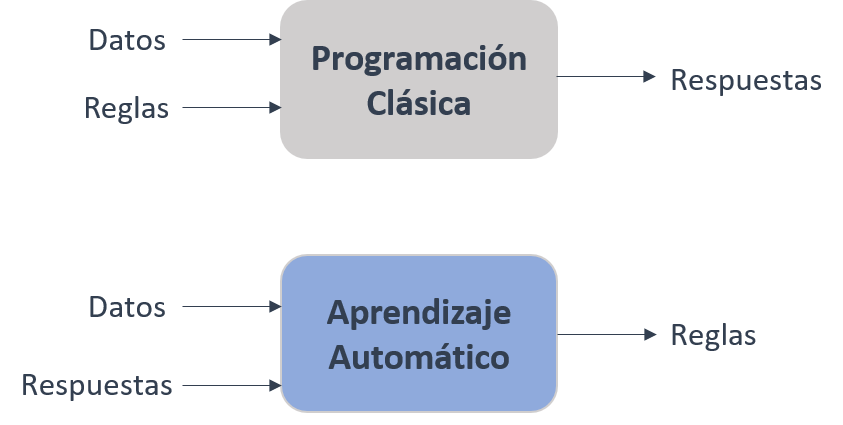
\includegraphics[width=3in]{Graphics/PCvsML.png}
	
	\caption{ \small{Programación clásica frente al aprendizaje automático.}}
	
	\label{PCvsML}
	
\end{figure}


El objetivo en el aprendizaje automático es seleccionar una función o hipótesis que se ajuste de manera óptima a ejemplos futuros o nuevos. Los parámetros de la función se ajustan durante el entrenamiento mediante un algoritmo de optimización conocido como descenso del gradiente. En esencia, transforma los datos de entrada a una salida que tiene una representación significativa, mediante un proceso llamado \textbf{aprendizaje}. 

Las tareas en este terreno, usualmente se describen en términos de cómo se procesa la entrada al sistema. Por lo general, se expresa como un vector $x \in \mathbb{R}$ donde cada componente del mismo constituye una característica. Por ejemplo, las características de una imagen pueden ser los valores de sus píxeles. Un sistema de aprendizaje automático se basa en un proceso de \textbf{entrenamiento} en lugar de ser programado explícitamente. Gracias a ello, permite encontrar una estructura estadística en los datos de entrada que dará lugar a nuevas reglas para automatizar la tarea en cuestión. En la siguiente sección se incluyen algunas tareas que se pueden resolver con técnicas de este dominio y que serán mencionadas a lo largo del documento. 

\subsection{Tareas de ML}\label{1-MLtareas}

Una tarea de aprendizaje automático es el tipo de predicción o inferencia que se realiza, en función del problema o la pregunta que se formula, y los datos disponibles. Las mismas se basan en patrones que pueden aparecer en los datos en lugar de programarse explícitamente. A continuación se muestran algunas de ellas.

\subsubsection{Clasificación}\label{1-Clasif}
 Su objetivo es clasificar la entrada del programa en una de las $k$ categorías posibles según el problema. Para resolverlo, el algoritmo de aprendizaje produce una función $f:\mathcal{R}^n \rightarrow \{1, ..., k\}$. Existen otras variantes de clasificación, por ejemplo, cuando $f$ devuelve una función de distribución de probabilidad sobre las $k$ categorías \cite{BengioGood}.
 
 \subsubsection{Regresión}\label{1-Regres}
 El algoritmo de aprendizaje reporta una función $f: \mathcal{R}^n \rightarrow \mathcal{R}$ para predecir un valor numérico a partir de la entrada. Un ejemplo de regresión es la predicción de los precios futuros en el mercado \cite{BengioGood}.

\subsubsection{Traducción automática}\label{1-TradAut}
 Del inglés \textit{machine translation}. La entrada consiste en una secuencia de símbolos en un determinado lenguaje, y el algoritmo la convierte a una secuencia de símbolos pero de otro lenguaje \cite{BengioGood}. Comúnmente se aplica en lenguajes naturales, por ejemplo para traducir del inglés al francés \cite{SutskeverSeq2seqNN, BahdanauAlignTrans}.
 
 \subsubsection{Detección de anomalías}\label{1-DetAnom}
 
 Es la identificación de elementos raros, eventos u observaciones que generan sospechas al diferenciarse significativamente de la mayoría de los datos. Normalmente, los datos anómalos se pueden conectar a algún tipo de problema o evento raro como, por ejemplo, fraude bancario, problemas médicos, defectos estructurales, equipo defectuoso, etc \cite{BengioGood}.
 
 %\subsubsection{Denoising}\label{1-Denois}
 
 %En este tipo de tareas, la entrada $x$ se altera mediante un proceso que añade ruido a la información contenida en sus valores, obteniendo así $\tilde{x} \in \mathcal{R} $. El algoritmo debe predecir $x$ a partir de su versión $\tilde{x}$, o más general, predecir la distribución de probabilidad condicional $p(x| \tilde{x})$.
 
 \subsubsection{Estimación de densidad(función de probabilidad)}\label{1-EstimDen}
 
En el problema de estimación de densidades, el algoritmo aprende una función $p_{model} : \mathbb{R}^2 \rightarrow \mathbb{R}$ de donde $p_{model}(x)$ se interpreta como la función de densidad (si $x$ es continuo) o una función de probabilidad (si $x$ es discreto) en el espacio donde se encuentran los elementos de entrada. Esta tarea permite capturar explícitamente una distribución, que además, podrá ser usada en otros fines. Por ejemplo, si se tiene una función de probabilidad ya estimada $p(x)$, la misma se puede usar para obtener un valor faltante $x_i$ a partir del resto de valores ya conocidos $x_{-i}$, dado por $p(x_i| x_{-i})$. 

\subsubsection{Reducción de dimensión}\label{1-RedDim}

Se define como una forma de convertir un conjunto de datos de dimensiones elevadas en un conjunto de datos de dimensiones menores, asegurando que la información proporcionada sea similar en ambos casos. Esta técnica es especialmente útil como paso intermedio en los modelos predictivos, ya que son conjuntos de datos que contienen un elevado número de características de entrada, y hace más complicada su función. Ejemplo de ello son los modelos \textit{autoencoders} que se abordan en este trabajo \cite{Chollet}.

\subsubsection{Extracción de características}\label{1-ExtCar}
Consiste en utilizar las representaciones aprendidas por un programa entrenado previamente para extraer características interesantes en nuevas muestras o datos. Básicamente, es un proceso de reducción de dimensión mediante el cual un conjunto inicial de datos se reduce a grupos más manejables para su procesamiento. Se usan para tareas de clasificación de imágenes donde el conjunto de datos es pequeño \cite{Chollet}.\\


Existen además otros tipos de tareas cuya solución es posible en este ámbito. Las listadas anteriormente son una muestra importante que están relacionadas con la investigación realizada en este trabajo.   

\subsection{Ramas dentro del aprendizaje automático}
\label{1-MLramas}

 Previamente se presentaron varios tipos de tareas específicas del aprendizaje automático. La definición de las mismas está relacionada con las características y procesamiento de los datos de entrenamiento \cite{Chollet}. En términos generales, los algoritmos de ML se pueden clasificar como no supervisados o supervisados según el tipo de experiencia que se les permite tener durante el proceso de aprendizaje \cite{BengioGood}. Clásicamente dichos algoritmos se separan en tres categorías descritas a continuación.
 
 \subsubsection{Aprendizaje supervisado}\label{1-MLsupervisado}
 El algoritmo se entrena con variables que incluyen los valores que se desean predecir; a estos valores conocidos se les llama $"$ etiquetas $"$. Su objetivo es crear una función capaz de predecir el valor correspondiente a cualquier objeto de entrada válida después de haber visto una serie de ejemplos, los datos de entrenamiento. Para ello, tiene que generalizar las situaciones no vistas previamente a partir de los datos presentados. La salida de la función puede ser un valor numérico (como en los problemas de regresión) o una etiqueta de clase (como en los de clasificación).
 
 \subsubsection{Aprendizaje no supervisado}\label{1-MLnosupervisado}
 
 Consiste en encontrar patrones interesantes en los datos de entrada sin necesidad de observar cuál es la salida.  Por lo tanto, el  objetivo es extraer información significativa de los datos, los cuales carecen de etiqueta y cuya estructura es desconocida. Existen dos tipos de problemas característicos en el aprendizaje no supervisado: el agrupamiento o \textit{clustering}, y la reducción de dimensión \cite{Chollet}. El agrupamiento se encarga de crear conjuntos de objetos de características similares, mientras que la reducción
 de dimensión busca información redundante en los datos para reducir el número de variables y así mejorar el rendimiento computacional
 
 \subsubsection{Aprendizaje reforzado}\label{1-RL}
 El aprendizaje reforzado (\textit{reinforcement learning}, RL) es una forma de aprendizaje automático basado en un sistema de recompensas y castigos en el que un agente busca las decisiones óptimas para obtener la máxima recompensa tanto a corto como a largo plazo. A diferencia del aprendizaje no supervisado, el aprendizaje reforzado trata de maximizar la función de recompensa (\textit{reward function}) en lugar de encontrar ciertos patrones ocultos en un conjunto de datos no etiquetados. El aprendizaje reforzado se hace cargo de una gama cada vez más amplia de aplicaciones del mundo real: vehículos autónomos, robótica, gestión de recursos, educación, etc \cite{Chollet}.\\
 
 %Cada algoritmo de aprendizaje reforzado debe seguir una política (policy) para decidir qué  decisión tomar en función del estado en el que se encuentre. No obstante, esta política   puede no seguirse en la etapa de aprendizaje. Aquellos algoritmos cuya regla de actualización realiza la acción que traerá el máximo beneficio a pesar de que la política actual  restrinja dicha acción, se denominan algoritmos \textit{off-policy}.
 
 %TODO: Esto es porque en el estado del arte se menciona una aplicación con este algoritmo
 
 %Q-learning es un algoritmo off-policy de aprendizaje reforzado que busca la mejor acción dado  el estado actual. Se considera off-policy porque la función aprende de las acciones que están  fuera de la política actual, como por ejemplo las acciones aleatorias. El objetivo es aprender la  política que maximice la recompensa total. La Q de Q-learning viene de quality, que en este caso mide lo útil que ha sido una acción para ganar una recompensa futura
 
 Un problema importante en el aprendizaje automático en general, es la tensión entre la optimización y generalización. La \textbf{optimización} se refiere al proceso de ajustar un modelo para obtener el mejor rendimiento posible en los datos de entrenamiento (aprendizaje), mientras que la \textbf{generalización} se refiere a qué tan bien se desempeña el modelo entrenado en los datos que nunca ha visto antes. 
 
 El objetivo es obtener una buena generalización, pero si no es controlada es posible que el modelo se ajuste en función de sus datos de entrenamiento solamente. Los procesos y conceptos involucrados para lograr este equilibrio se argumentan en la siguiente sección.
 
 %MEJORAR TRANSICIÓN
 
 \section{Fundamentos del aprendizaje automático}
 
 En este apartado se presentan los fundamentos para comprender la forma en la que las máquinas aprenden. Para ello, se explican los conceptos de función de costo y el método de descenso por gradiente. Posteriormente, se muestran los principales errores o problemas que surgen a la hora de realizar un modelo de ML: la varianza (variance), el sesgo (bias), el sobreajuste (overfitting) y el subajuste (underfitting). Por último, se explican los pasos a seguir para desarrollar e implementar una solución con ML.
 
 \subsection{Aprendizaje}\label{1-Learning}
 
 El aprendizaje en un sistema de ML consiste en el ajuste de los parámetros de un modelo en función de los datos recibidos. Este conjunto de datos contiene variables tanto independientes como dependientes. Las variables  independientes (\textbf{características}) son aquellas usadas por el algoritmo para generar un modelo que prediga lo mejor posible las variables dependientes. Por otro lado, las variables dependientes (\textbf{etiquetas}) son el resultado de una correlación entre las variables independientes, por lo que deben ser predichas por el modelo implementado. 
 
 El modelo debe estar lo suficientemente ajustado a los datos de entrada, pero también debe tener la suficiente consistencia como para dar un buen resultado ante la introducción de datos diferentes. Para ello, el conjunto de datos se divide en 3 subconjuntos: los datos de entrenamiento (\textbf{training set}), con los que se entrenan los modelos candidatos; los datos de validación (\textbf{validation set}), para evaluar los modelos candidatos y seleccionar el mejor; y los datos de prueba (\textbf{test set}) para realizar una evaluación final del mejor modelo \cite{PeterNorvig}.
 
 Una vez se tienen los datos se establece una hipótesis, es decir, encontrar una ecuación que se aproxime lo mejor posible al comportamiento real del fenómeno que se está  modelando. Esta ecuación relaciona los datos de entrada y los parámetros del modelo con la salida y se conoce como \textbf{función de pérdida}. Se encarga de recopilar el error entre la variable dependiente que se quiere determinar y la hipótesis, en función de los parámetros del modelo.
 
 La diversidad de modelos y funciones de pérdida en ML obliga a encontrar soluciones para las funciones no-convexas, es decir, para aquellas que tienen más de un mínimo.  El método de \textbf{Descenso por Gradiente} aprovecha el cálculo de la derivada para encontrar los mínimos locales, ya que la derivada indica el valor de la pendiente en un punto determinado. El gradiente proporciona información sobre cuánto varía la función por cada unidad que varía cada variable en el punto considerado. Un gradiente positivo indica la dirección por la cual avanzar si se quisiera encontrar un máximo
 (Ascenso del Gradiente). En este caso, se explora el espacio en el sentido contrario al gradiente, ya que el objetivo es encontrar un mínimo de la función.
 
 \subsection{El error y los problemas de ajuste}\label{1-Ajuste}
 
 La precisión y la capacidad de generalizar son aspectos clave a la hora de realizar un modelo de ML solo que, lamentablemente, es imposible conseguir que un modelo esté libre de errores por completo. Comprender las principales fuentes de error ayuda a prevenir dos de los problemas más habituales en el ajuste de parámetros: el sobreajuste (\textbf{overfitting}) y el subajuste o falta de ajuste (\textbf{underfitting}).
 
 Los errores principales en la predicción de un modelo, y que están asociados al algoritmo empleado, son la varianza y el sesgo (bias). El error de varianza está relacionado con el grado en el que la función objetivo cambia según los datos de entrenamiento proporcionados. El error de sesgo es la diferencia entre los valores reales y la predicción que espera el modelo. El error total es una combinación de varianza y sesgo, por lo que para minimizarlo es imprescindible lograr una baja varianza y un bajo sesgo. Sin embargo, la estrecha relación entre la varianza y el sesgo hace que disminuir uno de ellos
 implique aumentar el otro.
 
 El subajuste (underfitting) se refiere a un modelo con un nivel de complejidad muy bajo que no tiene la precisión suficiente como para alcanzar un ajuste adecuado debido a su alto sesgo. Puede ocurrir cuando el conjunto de datos de entrenamiento no es suficiente, o cuando se utiliza un modelo lineal para ajustar datos no lineales. Por otra parte, el sobreajuste (overfitting) se produce cuando el nivel de complejidad es elevado y, por lo tanto, el modelo no tiene la capacidad de generalizar su comportamiento ante diferentes datos de entrada. Sucede cuando el modelo recoge el ruido de los datos de entrenamiento y, en consecuencia, aumenta mucho su varianza.
 
 \subsection{Etapas de un proyecto de ML}\label{1-etapas}
 
 Una vez presentados los principios básicos del ML, es conveniente conocer el procedimiento para dar solución a problemas reales usando estas técnicas. Un proyecto de ML no se centra únicamente en elegir un modelo y entrenarlo, sino que, como todo proyecto, cuenta con una serie de etapas o pasos a seguir para aumentar sus probabilidades de éxito. A continuación, se describen ocho etapas genéricas \ref{etapasML} para llevar a cabo un proyecto de ML.
 
  \begin{figure}[!h]
 	\centering
 	
 	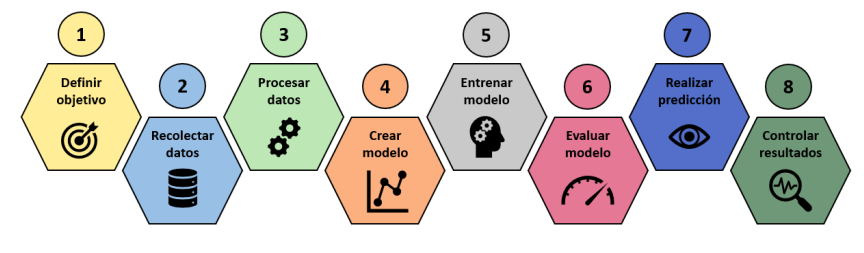
\includegraphics[width=4in]{Graphics/etapasML.png}
 	
 	\caption{ \small{Etapas genéricas de un proceso de ML.}}
 	
 	\label{etapasML}
 	
 \end{figure}

La primera etapa consiste en entender el problema que se quiere resolver, ya que gran parte de las decisiones tomadas a lo largo del proyecto dependerán de lo bien que se haya comprendido el contexto. Para ello es necesario definir unos objetivos claros, medibles y alcanzables en un período determinado de tiempo. En este punto se clasifica el problema (supervisado, no supervisado, etc.) e incluso se elige el tipo de modelo que se va a entrenar.

En la segunda etapa se define la cantidad y el tipo de datos necesarios, así como el origen de dichos datos. La calidad de los datos tiene un impacto directo en el funcionamiento del modelo. Por tal motivo, es necesario desarrollar una tercera etapa de tratamiento y procesamiento de los datos, cuyo objetivo es visualizar y analizar cuáles son las variables que mejor representan aquello que se quiere predecir. Además, los datos requieren un formato determinado para poder procesarse de la manera más sencilla posible. Para ello debe se debe tener en cuenta las características de la arquitectura empleada y la representación seleccionada para los datos. En esta tercera etapa se incluyen dos procedimientos que tienen lugar en este trabajo y consisten en lo siguiente: 
	
	\begin{description}
		\item[Vectorización:] todas las entradas y etiquetas deben ser vectores con valores reales.
		
		\item[Normalización:] una vez vectorizados los datos, deben cumplir además que sus valores se encuentren en el intervalo $[0, 1]$.
	\end{description}

Una vez hecho esto, se divide el conjunto de datos en los 3 subconjuntos mencionados anteriormente. 

Aunque en el primer paso ya se conoce el tipo de problema, es en la etapa cuatro donde se define por completo el modelo que mejor se ajusta al problema: regresión lineal, árboles de decisión, red neuronal, k-vecinos más cercanos, etc. La solución propuesta en este trabajo contempla dos modelos de redes neuronales conocidos como \textit{autoencoder} y \textit{variational autoencoder}.

La quinta etapa se dedica al entrenamiento del modelo a partir de los datos de entrenamiento. Los parámetros se ajustan automáticamente por el algoritmo seleccionado a medida que se entrena el modelo. En la etapa número seis se verifica la precisión del modelo mediante la introducción de los datos de prueba, que son datos distintos a los del conjunto de entrenamiento. También se evalúan los errores que hacen que el modelo no generalice bien con el fin de elegir la solución más conveniente: adquirir más datos, usar un modelo más simple, usar uno más complejo, comprender mejor el problema, etc. A esta etapa también se la conoce como Parameter Tuning (configuración de parámetros), pues consiste en ajustar los parámetros del modelo para mejorar los resultados obtenidos.

Cuando se alcanza el nivel de error deseado, el modelo queda validado y puede pasarse a la penúltima etapa, que es la unión entre la simulación y el mundo real. Se trata de integrar el modelo en un sistema real con el que pueda comunicarse. Por último, la etapa número ocho pone fin al proceso con la monitorización de los resultados. Es necesario asegurar que el modelo aporta un alto valor predictivo y, lo más importante, que
cumple con los objetivos marcados en la primera etapa.

El aprendizaje automático comenzó a florecer en la década de 1990. Según \textit{Chollet et al.} \cite{Chollet}, una tendencia impulsada por la disponibilidad de \textit{hardware} más rápido y también conjuntos de datos de mayor dimensión. A diferencia de la estadística, el aprendizaje automático tiende a tratar con conjuntos de datos más grandes y complejos (como un conjunto de millones de imágenes, cada una de ellas formada por decenas de miles de píxeles) cuyo análisis estadístico clásico, como el análisis bayesiano, no sería practicable. Como resultado, el aprendizaje automático, y especialmente el aprendizaje profundo, exhibe poca teoría matemática. Esta disciplina, conocida en inglés como \textit{deep learning}, se introduce en la siguiente sección.


  
 \section{Aprendizaje profundo}\label{1-DeepLearn}
 
 Existe un área específica del aprendizaje automático llamada aprendizaje profundo (\textit{deep learning}), que se basa en algoritmos de aprendizaje en múltiples niveles de representación y de abstracción con el fin de modelar relaciones más complejas entre los datos. Los niveles se corresponden con distintos niveles de conceptos, y a cada uno, le corresponde una capa dentro de una secuencia formada por capas. Esta idea de representaciones sucesivas es lo que da el nombre de “profundo” a este tipo de aprendizaje, siendo la profundidad del modelo el número de capas que contiene \cite{deng2014deep}.
 
 En el aprendizaje profundo, estas representaciones por capas forman una red neuronal (\textit{neural network}) que constituyen un conjunto estructurado de neuronas \ref{RedNeuronal}. Estos términos provienen de la neurobiología ya que estas redes se inspiran en el funcionamiento del cerebro. Las capas están formadas por un número determinado de neuronas, donde cada neurona recibe información de la capa anterior por medio de estímulos externos a través de sus conexiones de entrada. 
 
 Las neuronas realizan cálculos internamente y sobre ellas se usa una función de activación para propagar la salida de los nodos o neuronas de la capa actual hacia la siguiente capa. Se trata de funciones que producen la activación de la neurona. Este tipo de funciones permiten incorporar la modelación de relaciones no lineales en los datos de entrada a la red.
 
 La función de activación \textit{relu} es la más utilizada en el aprendizaje profundo \cite{Chollet} y se define como $ReLU(z) = max(0, z)$. Otro ejemplo es la función $sigmoid$ que se determina mediante la función $\sigma(z) = \frac{1}{1 + e^{-z}}$. Ambas funciones se emplearon en los modelos implementados en este trabajo.
 
 
 
 % devuelven un valor de salida que se transmite a las neuronas de la capa siguiente. En la última capa, la salida es la predicción buscada \cite{Chollet}.
 
 \begin{figure}[!h]
 	\centering
 	
 	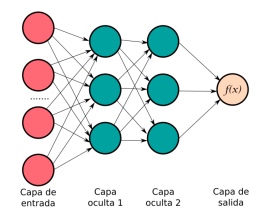
\includegraphics[width=2.55in]{Graphics/redNeuronal.png}
 	
 	\caption{ \small{Arquitectura básica de una red neuronal.}}
 	
 	\label{RedNeuronal}
 	
 \end{figure}

%Sin embargo, para llegar a una buena predicción, la red debe ser capaz de minimizar el error entre la predicción y el valor esperado mediante el autoajuste de los parámetros del modelo.

La especificación de lo que hace una capa con sus datos de entrada se almacena en los \textbf{pesos} de la capa, que en esencia, son un conjunto de números. En términos técnicos, se dice que la transformación implementada por una capa se \textbf{parametriza} por sus pesos (los pesos también se denominan parámetros de una capa) \ref{RedLoss}. En este contexto, aprender significa encontrar un conjunto de valores para los pesos de todas las capas en una red, de modo que la red transforme correctamente la entrada a su objetivo asociado.

El aprendizaje ocurre al extraer lotes (\textit{batches}) aleatorios de muestras de datos y sus
etiquetas, y calcular el gradiente de los parámetros de la red con respecto a la pérdida en el lote. Luego, los parámetros de la red se mueven un poco en el
dirección opuesta al gradiente.

Para controlar el valor de la salida de la red, se mide qué tan lejos se encuentra la misma de la respuesta deseada mediante la \textbf{función de pérdida}, también llamada función objetivo. La función de pérdida toma las predicciones de la red y el verdadero objetivo (lo que deseaba que produjera la red) y calcula una medida de distancia, capturando qué tan bien ha funcionado la red para cada uno de los ejemplos de entrada. 

 Todo el proceso de aprendizaje es posible gracias al hecho de que la red neuronal constituyen cadenas de operaciones vectoriales \textbf{diferenciables} Chollet et al. \cite{Chollet} y, por lo tanto, es posible aplicar la regla de derivación de la cadena para encontrar la función de gradiente que transforme a los parámetros actuales y al lote actual de datos, a un valor de gradiente.

 \begin{figure}[!h]
	\centering
	
	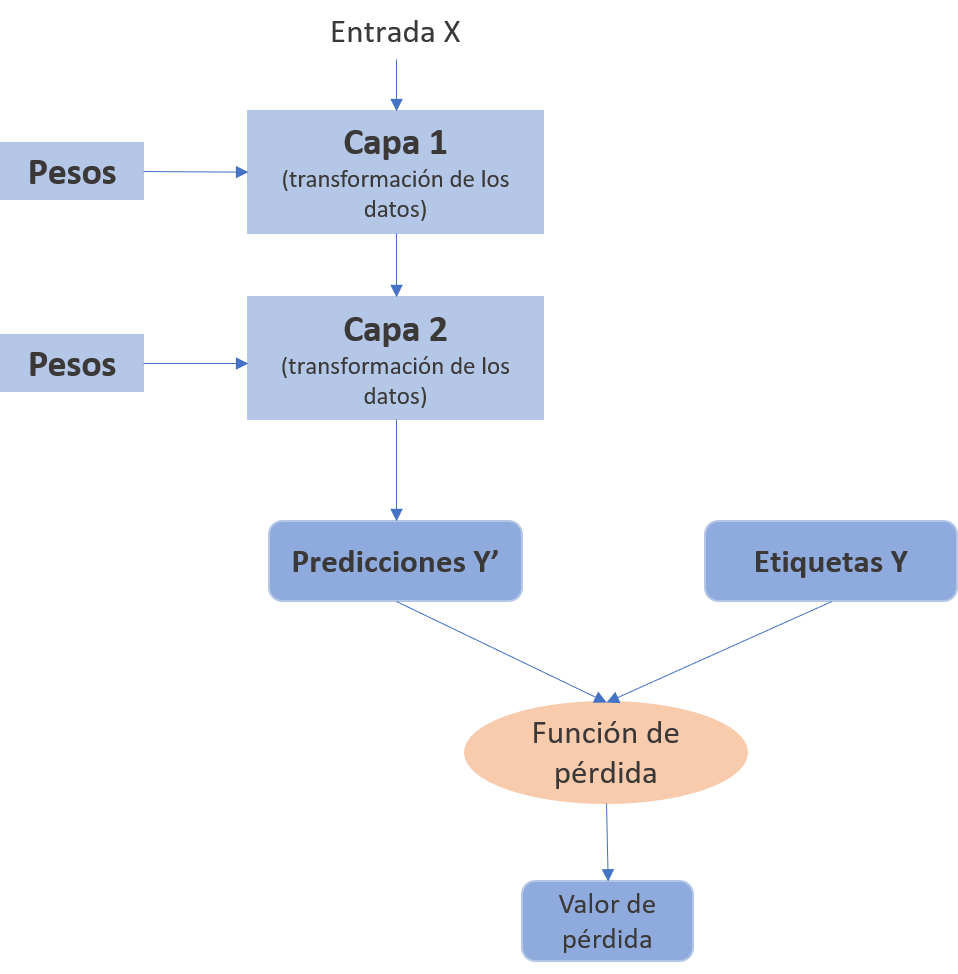
\includegraphics[width=3.8in]{Graphics/redLoss.png}
	
	\caption{ \small{Red neuronal parametrizada por sus pesos y con función de pérdida para evaluar la calidad de la salida.}}
	
	\label{RedLoss}
	
\end{figure}

El truco fundamental en el aprendizaje profundo es utilizar esta medida como una señal de \textbf{retroalimentación} para ajustar el valor de los pesos, en una dirección que reducirá la medida de pérdida para el ejemplo actual. Este ajuste es el trabajo del \textbf{optimizador}, que implementa lo que se conoce como algoritmo \textbf{Backpropagation} \cite{Chollet}.

En la literatura existen varios algoritmos de optimización basados en el descenso por gradiente. Entre los más conocidos se encuentran los algoritmos de optimización \textit{Adam} y \textit{RMSProp} \cite{BengioGood}. Este último utiliza una tasa de aprendizaje adaptativa en lugar de tratar la tasa de aprendizaje como un hiperparámetro. Esto significa que la tasa de aprendizaje cambia con el tiempo.  


\begin{figure}[!h]
	\centering
	
	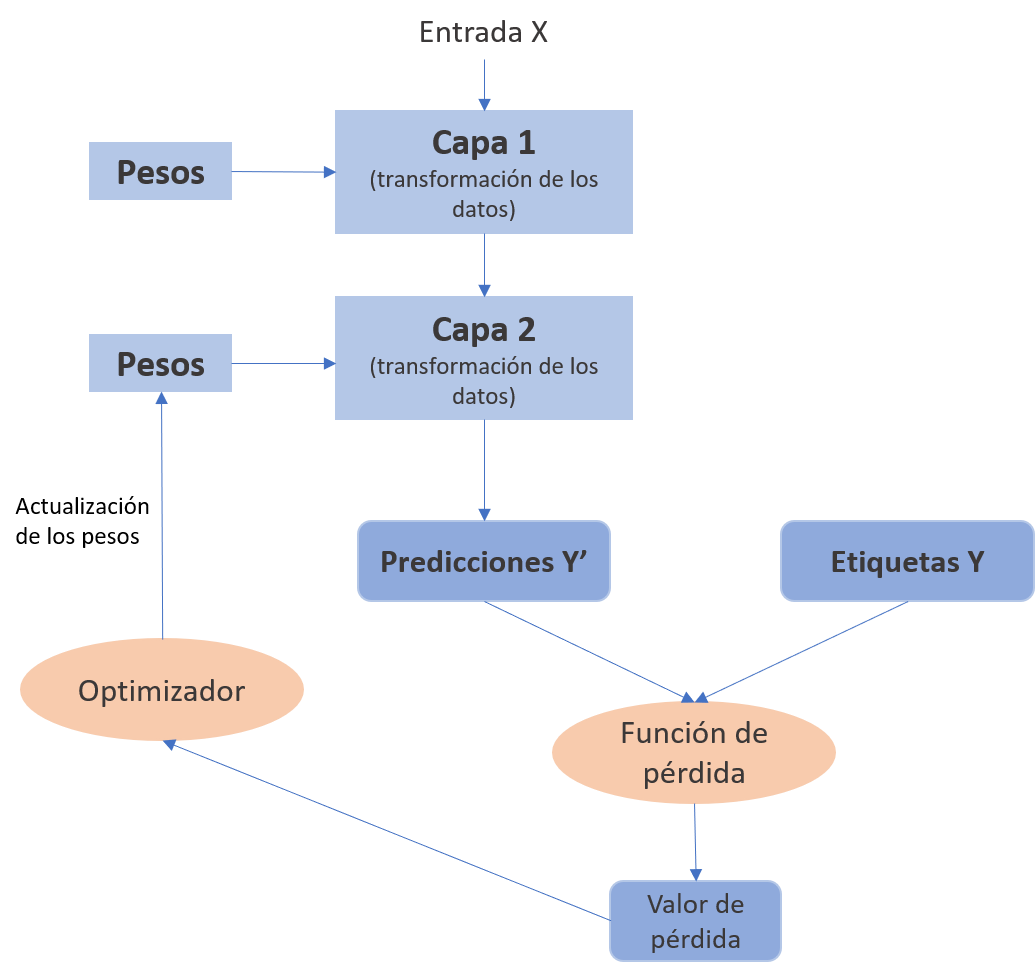
\includegraphics[width=3.8in]{Graphics/redBP.png}
	
	\caption{ \small{La pérdida es usada como señal de retroalimentación para el ajuste de los parámetros de la red.}}
	
	\label{RedBP}
	
\end{figure}

Inicialmente, los pesos de la red toman valores aleatorios mediante un proceso conocido como inicialización aleatoria (\textit{random initialization}).  Naturalmente, su salida está lejos de lo que debería ser, y en consecuencia, la medida de pérdida es muy alta. Pero con cada ejemplo que procesa la red, los pesos se ajustan un poco en la dirección correcta, y la pérdida disminuye. Este es el \textbf{ciclo de entrenamiento}, que, repetido las veces suficientes, produce valores de pesos que minimizan la función de pérdida. Las iteraciones comprendidas en el ciclo se conocen como épocas (\textbf{epochs}) del proceso de entrenamiento. Una red con una pérdida mínima es aquella donde la salida es lo más parecido posible al objetivo.
 %Nuevamente, es un mecanismo simple que, una vez escalado, termina pareciendo mágico.
 
 \subsection{Tipos de redes neuronales}\label{1-NN}
 
Una característica importante de algunas redes neuronales, como las \textbf{redes neuronales densamente conectadas}, es que no tienen memoria. Cada entrada a la misma se procesa de forma independiente, sin que se mantenga ningún estado de una entrada a otra. Para procesar una secuencia o una serie temporal de puntos en los datos, es necesario introducir de una vez la secuencia completa a la red. Tales redes se llaman redes unidireccionales (del inglés  \textit{feedforward} ). 

%feedforward -> unidireccionales

La predicción de datos secuenciales supone un problema en ML, ya que usualmente se analizan casos aislados como una imagen o un carácter que se desea clasificar. Sin embargo, lo que una persona entiende al ver una película o al mantener una conversación, se basa en conocimientos anteriores que van adquiriendo sentido con cada instante que transcurre. Las redes neuronales recurrentes (recurrent neural networks, RNN) son un tipo de algoritmo de aprendizaje profundo que se encarga de resolver este problema mediante el procesamiento de datos secuenciales \cite{BengioGood}.

Las RNN en lugar de tener una estructura por capas como las redes neuronales convencionales, poseen una estructura cíclica donde la salida de un estado pasa a ser la entrada del estado siguiente \ref{RNN} . Esto permite detectar dependencias temporales, es decir, dotar a la red de memoria (estado oculto o hidden state) para que retenga la información sobre lo calculado en la etapa anterior. De esta forma, utiliza los mismos parámetros para cada entrada, reduciendo así la complejidad de la red \cite{RNNVinyals}.

\begin{figure}[!h]
	
	\centering
	
	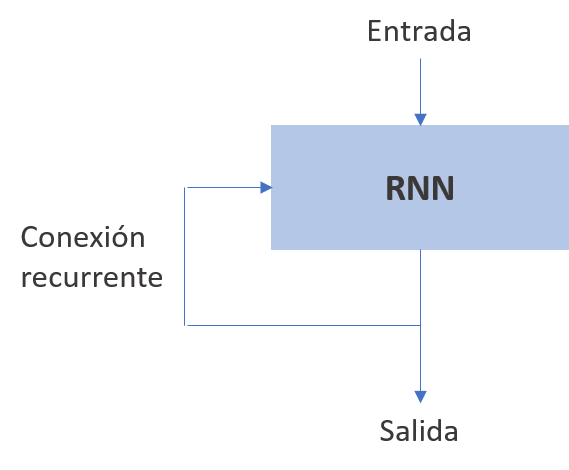
\includegraphics[width=2.3in]{Graphics/RNNConnection.png}
	
	\caption{\small{Esquema básico de una RNN}}
	\label{RNN}
	
\end{figure}

Como parte del amplio estudio realizado en esta tesis, se revisaron trabajos que incluyen la utilización de este tipo de redes \cite{SutskeverSeq2seqNN, PointerNVinyals}. Además, como se había mencionado, la solución propuesta en esta investigación contempla dos modelos de redes neuronales conocidos como \textit{autoencoder} y \textit{variational autoencoder}. Este último forma parte de los modelos generativos dentro del aprendizaje automático y se abordará en la siguiente sección.


\section{Modelos generativos}\label{1-GenModel}

Los modelos generativos constituyen un área del aprendizaje automático que se dedica a encontrar la distribución $P(X)$, definida sobre los puntos $X$ de un espacio $\mathcal{X}$ de gran dimensión. Por ejemplo, las imágenes son un tipo de datos muy popular empleadas en modelos generativos \cite{VAETutorial}, donde cada una puede tener miles o millones de píxeles. En este caso la tarea del modelo generativo es capturar de alguna manera las dependencias entre píxeles, por ejemplo, que los píxeles con colores similares se encuentren cercanos entre sí.

Un tipo sencillo de modelo generativo permite calcular numéricamente $P(X)$. En el caso de las imágenes, los valores $X$ que parecen imágenes reales deberían tener una alta probabilidad, mientras que las imágenes que posean determinado ruido aleatorio deberían tener una probabilidad baja.

 Su idea principal se basa en generar puntos nuevos, parecidos a los del conjunto de datos inicial, pero no exactamente los mismos. Formalmente, el objetivo es aprender un modelo $P$ para muestrear puntos $X$ que satisfacen una distribución no conocida $P^{*}(X)$, de forma tal que $P$ sea lo más parecido posible a $P^{*}$.
 
 Los \textit{variational autoencoders} constituyen un ejemplo clásico dentro de la familia de modelos generativos. Sus buenas propiedades de aproximación, y el pequeño error introducido con ella, aportan gran capacidad de generación al modelo. Además, son capaces de comprimir los datos de entrada en una representación con menos información, conocida como representación latente. Es por ello que su estudio resulta de gran interés en este trabajo.
 
  En el capítulo \ref{chapter:REV-LL} se profundizará en la teoría detrás del VAE y posteriormente, en el capítulo \ref{chapter:Solution} se explicará en qué consiste su uso para codificar soluciones del VRP a un vector real o vector latente. Antes de llegar a esos puntos, primeramente, se analizarán los modelos de variable latente en la siguiente sección. 
 
 
 %Dicho vector codificado, conocido también como vector de contexto o vector latente es analizado durante esta investigación, en cuanto a las propiedades y características capturadas de la distribución de entrada inicial. 
 


\subsection{Modelos de Variable Latente}\label{1-latentVarModel}

Los modelos matemáticos que tratan de explicar las variables observadas en términos de variables latentes se llaman modelos de variables latentes. Para comprender mejor en qué consisten, se presenta un ejemplo mediante el problema de la generación de imágenes referentes a dígitos escritos a mano.

 Durante el proceso, el modelo primeramente decide qué dígito va a generar antes de asignar valores a cualquiera de los píxeles. Este tipo de decisiones se conocen formalmente como variable latente. Es decir, el modelo muestrea aleatoriamente un dígito $z$ del conjunto $[0, ..., 9]$ y luego se asegura de que todos los trazos coincidan con el mismo. En este caso $z$ es la variable latente. A continuación se define formalmente.
 
 Si $z$ es un vector de variable latente en un espacio de dimensión elevada $\mathcal{Z}$, $z$ puede ser muestreado de acuerdo a la función de densidad probabilística $P(z)$ definida sobre $\mathcal{Z}$. También se tiene a $f(z; \theta)$ como una familia de funciones deterministas parametrizadas por un vector $\theta$ que pertenece a un espacio $\Theta$, donde $f: \mathcal{Z} \times \Theta \rightarrow X$.
 
  Como $f$ es determinista y $\theta$ no lo es, entonces $f(z; \theta)$ es una variable aleatoria en el espacio $\mathcal{X}$. La idea es optimizar los parámetros $\theta$ de forma tal que se pueda muestrear $z$ a través de $P(z)$, teniendo en cuenta que $f(z; \theta)$ serán como los elementos $X$ del conjunto de datos. 
 
 Matemáticamente el objetivo es maximizar la probabilidad de cada punto $X$ en el conjunto de entrenamiento a lo largo del proceso generativo, de acuerdo a:
 
 \begin{equation}
 	P(X) = \displaystyle{\int} P(X| z; \theta)P(z)dz
 \end{equation} 
 
 Aquí, $f(z; \theta)$ se reemplazó por una distribución $P(X| z; \theta)$, lo que permite hacer explícita la dependencia de $X$ con $z$ utilizando la ley de probabilidad total. En los modelos VAEs la función de distribución empleada generalmente  es Normal, es decir $P(X|z;\theta) = \mathcal{N}(X|f(z; \theta), \sigma^2*I)$. La media se define a partir de $f(z, \theta)$ y la covarianza como la matriz identidad $I$ multiplicada por un escalar $\sigma$ (que es un hiperparámetro de la red neuronal). Estas sustituciones son necesarias para formalizar la intuición de que las variables $z$ necesitan ser parecidas a algún $X$ \cite{VAETutorial}. 
 
 En general, y particularmente al principio del entrenamiento, el modelo no producirá resultados que sean idénticos a cualquier $X$ en particular. Al tener una distribución gaussiana, se usa descenso por gradiente para aumentar la probabilidad $P(X)$, haciendo que $f(z; \theta)$ se aproxime a $X$ para algún $z$, es decir, permitiendo gradualmente que los datos de entrenamiento sean más probables bajo el modelo generativo.\\
 
 Con este primer capítulo se presentó una introducción al aprendizaje automático. En esencia, se ofrecieron los principios y conceptos teóricos más importantes del área que fundamentan el trabajo realizado en esta tesis y muchas de las decisiones tomadas. Aprender a resolver automáticamente problemas complejos como el VRP, podría implicar el próximo salto en el desarrollo de la optimización combinatoria.  
 
 La solución propuesta en este trabajo para codificar soluciones del VRP a vectores de un espacio continuo, tiene lugar en este terreno. Específicamente mediante el uso de los modelos \textit{autoencoders} y \textit{variational autoencoders}. En el próximo capítulo se profundiza en la definición teórica de estos modelos de redes neuronales, así como también las aplicaciones de los mismos en problemas de codificación similares. También se exponen una serie de técnicas de ML que resultan de gran interés para esta investigación. 
 
 
 
 
 




 


\chapter{Preliminares}\label{chapter:REV-LL}

Este trabajo pretende implementar un sistema que resuelva instancias de VRP en cualquiera de sus variantes con el menor trabajo humano posible. En este capítulo se presentan los principales elementos de la investigación realizada para lograrlo.

Primeramente se comienza con una visión general del problema de enrutamiento de vehículos (VRP) y algunas de sus variantes con la sección \ref{2-VRPintro}. Se explica cómo describir a partir de código una solución de VRP.

 En \ref{2-Libr} se muestran las bibliotecas de clases existentes hasta el momento que pueden ser utilizadas para encontrar soluciones a instancias de VRP.
 
En \ref{2-Hector} se explica cómo crear un Árbol de vecindad a partir de una solución inicial y un criterio de vecindad. Este árbol es utilizado para obtener la cardinalidad de vecindades y realizar una exploración de dos fases que utiliza técnincas estadísticas.

En \ref{2-JJ} se expone el concepto de Grafo de evaluación y cómo es esto utilizado para evaluar soluciones de forma eficiente y automática.

En \ref{2-Heidy} se presenta un mecanismo para explorar vecindades de forma automática a partir de combinaciones de cualesquiera estrategias de exploración y selección.

Finalmente en \ref{2-Lisp} se describe brevemente algunas características y funcionalidades del lenguaje Common Lisp que resultaron especialmente útiles para el desarrollo del sistema.


%\newpage

\section{Problema de Enrutamiento de Vehículos}\label{2-VRPintro}
La primera referencia al VRP fue hecha por Dantzing y Ramser en \cite{Ramsin1959} en el año 1959. Se propone una formulación matemática, una aproximación algorítmica y se describe una aplicación real entregando gasolina a varias estaciones de servicio. 

En su versión más simple, el problema consta de una flota de vehículos que salen de un depósito y deben satisfacer las demandas de una serie de clientes. El objetivo es encontrar una distribución de caminos a asignar a los vehículos de forma que se optimice determinada métrica (tiempo, combustible, etc). Con más de 50 años de estudios se ha ramificado en una inmensa cantidad de variantes entre las que se pueden contar las siguientes:

\begin{itemize}
	\item CVRP - VRP con restricciones de capacidad. Cada vehículo tiene una capacidad que no debe ser excedida.
	\item VRPTW - VRP con ventanas de tiempo. Cada cliente posee un período de tiempo fijo durante el cual puede ser atendido.
	\item VRPPD - VRP con recogida y entrega. Los bienes deben ser entregados y recogidos en cantidades fijas.
	\item MDVRP - VRP con múltiples depósitos. Se cuenta con múltiples depósitos desde los que pueden salir los vehículos.
\end{itemize}

Esta es una familia de problemas NP-Duros, por lo las soluciones exactas no son factibles para instancias de grandes tamaños. Para buscar aproximaciones a la solución se utilizan heurísticas y metaheurísticas. Se destaca la búsqueda local como metaheurística que ha dado muy buenos resultados y es la seleccionada en el presente trabajo como se explica en \ref{2-Local}.

\subsection{Representación de soluciones del VRP}\label{2-Sol}
Las soluciones son representadas (en su versión más simple) como una serie de listas de clientes denominadas rutas.
Si se define a $P_1$ como un problema clásico que consta de 6 clientes: $[c_1, c_2, c_3, c_4, c_5, c_6]$, entonces una solución $s_1$ se puede definir como:

\begin{equation}
s_1 = [(c_2,c_3), (c_1,c_4,c_5), (c_6)]
\end{equation}

En $s_1$ se representa una solución con tres rutas. El vehículo perteneciente a la primera ($r_1$) ruta visita a $c_2$ y $c_3$, el vehículo de la segunda ruta ($r_2$) visita a $c_1$, $c_4$ y $c_5$ y el de la tercera ($r_3$) sólo visita a $c_6$.


\subsection{Metaheurísticas de búsqueda local}\label{2-Local}
Los algoritmos basados en búsquda local son aquellos en que se define una solución inicial y a partir de determinado criterio de vecindad se busca la solución óptima iterando por los vecinos de la vecindad formada por dicho criterio. A continuación se muestran algunos ejemplos de criterios de vecindad:

\begin{enumerate}
	\item Cambiar de posición a un cliente dentro de su ruta.
	\item Mover a un cliente de ruta.
	\item Intercambiar dos clientes de posición.
	\item Cambiar vehículo de ruta.
	\item intercambiar dos subrutas entre sí.
	\item invertir orden de una subruta. 
\end{enumerate}

Los criterios de vecindad dependen también de la variante del problema sobre la que se trabaje. Por ejemplo, el criterio de \textbf{"Cambiar vehículo"} no tiene sentido para el problema $P_1$ pues en este todos los vehículos son iguales.

Estas operaciones pueden ser obtenidas a partir de un subconjunto de operaciones más simples a las que se denomina operaciones elementales. Entre las operaciones elementales se encuentran: \textbf{selección de ruta}, \textbf{selección de cliente} e \textbf{inserción de cliente} que comunmente se representan con los símbolos \textit{r}, \textit{a} y \textit{b} respectivamente. 

Por ejemplo, \textbf{intercambiar dos clientes de posición} puede ser realizado a partir de dos \textbf{selección de ruta}, dos \textbf{selección de cliente} y dos \textbf{inserción de cliente}.

La importancia de las operaciones elementales para la implementación del sistema se explicarán en con más profundidad en \ref{label}.

A partir de un criterio y una solución inicial se pueden generar nuevas soluciones. El proceso de obtención y selección de nuevas soluciones se denomina exploración de la vecindad. Mientras más grande la vecindad es más probable encontrar mejores soluciones, pero esto puede requerir una gran cantidad de tiempo. Por tanto, las estrategias a seguir durante la exploración son un factor vital a tener en cuenta para la implementación del sistema y se explicarán en \ref{2-Hector} y \ref{2-Heidy}. Además, a la hora de comparar el costo entre dos soluciones es necesario evaluarlas, lo cual posee también un costo computacional considerable. Para la evaluación de soluciones se tiene el Grafo de evaluación explicado en \ref{2-JJ}.

\section{Vías de solución existentes}\label{2-Libr}
Una buena herramienta para resolver problemas de VRP en la actualidad es la biblioteca OR-Tools (Google Optimization Tools). Un software de código abierto útil para problemas de optimización combinatoria entre los que se encuentra el Problema de Enrutamiento.

\section{Árbol de vecindad}\label{2-Hector}
La exploración de vecindades puede ser ineficiente y difícil de programar. La idea que se propone es utilizar técnicas estadísticas para analizar cuáles son las mejores regiones de las vecindades para intensificar la búsqueda en estas.

Buscando aplicar dichas técnicas estadísticas es necesario saber la cardinalidad de las vecindades y separarlas en regiones. Para lograr esto de forma eficiente (sin iterar por todos los elementos de una vecindad) se propone la creación de un Árbol de vecindad. El Árbol de vecindad utiliza un concepto de $solucion$ diferente al explicado en \ref{2-Sol}. Previamente se definió una solución de VRP en su forma más trivial como una lista de caminos conformados a su vez por la lista de clientes que se visitan en cada uno, por ejemplo:

\begin{equation}
s_1 = [(c_2,c_3), (c_1,c_4,c_5), (c_6)]
\end{equation}

Con el propósito de contar la cantidad de soluciones que tiene una vecindad, pierde importancia saber qué clientes se visita en cada ruta, en cambio sólo es necesario conocer la cantidad de clientes visitados en cada una. A este tipo de solución se le denomina solución de conteo y aplicado a $s_1$ daría como resultado:

\begin{equation}
sc_1 = [2, 3, 1]
\end{equation}

Teniendo una solución inicial, todas las soluciones de una vecindad pueden ser obtenidas aplicando sobre esta el criterio de vecindad en cuestión, con todos sus valores posibles. A la asignación de valores de un criterio de vecindad sobre una solución se le llamará una instanciación de dicho criterio. Por ejemplo, dado el criterio \textbf{mover cliente} dado por: 

\begin{itemize}
	\item Seleccionar ruta (r1).
	\item Seleccionar cliente (c1) de ruta (r1).
	\item Seleccionar ruta (r2).
	\item Insertar cliente (c1) en ruta (r2).
\end{itemize}

Un ejemplo de instanciación de este criterio sobre la solución $s_1$ se presenta como:

\begin{itemize}
	\item $r_1 = 1$ $\rightarrow$ $r_1$ es la ruta de la que el cliente $c_1$ es extraído.
	\item $c_1$ = 1 $\rightarrow$ $c_1$ es el primer cliente de la ruta.
	\item $r_2 = 2$ $\rightarrow$ $r_2$ es la ruta en la que el cliente $c_1$ será insertado.
	\item $c_1$ = 2 $\rightarrow$ $c_1$ es insertado en la posición 2 de la ruta seleccionada.
\end{itemize}

A cada vecino de un criterio se le puede hacer corresponder una instanciación del mismo y por tanto, encontrar la cardinalidad de una vecindad es similar a encontrar el número de instanciaciones posibles del criterio asociado.

Al generar las distintas instanciaciones de un criterio de vecindad para
una solución dada se cumple que muchas de estas comparten una secuencia común de operaciones instanciadas. La estrategia propuesta se basa en agrupar aquellos criterios instanciados para los cuales dicha secuencia común comience en la primera operación de los mismos, pues de esta forma el resto de las operaciones de tales criterios instanciados no se ven afectadas, y contar para cada una de estas el número de posibles secuencias de operaciones instanciadas que unidas con la secuencia común forman un criterio instanciado.

Al computar la cardinalidad de una vecindad del VRP, se utiliza una estrategia recursiva que consiste en contar para una operación el número de secuencias de operaciones instanciadas que se pueden formar con el resto de las operaciones del criterio, así como combinar las mismas con las posibles instanciaciones de la operación actual aprovechando que para las operaciones modificadoras estas secuencias son comunes a todas las posibles instanciaciones de las mismas.

Es posible utilizar este algoritmo, para almacenar toda la información necesaria para cualquier procesamiento posterior sobre dicha vecindad en una estructura arbórea que será llamada árbol de vecindad y que constituye una representación de la vecindad en cuestión. En \ref{fig:neigh-tree} se muestra una representación del árbol de vecindad asociado a l criterio \textbf{mover cliente} ($rarb$). Cada nodo del árbol, representa una operación de vecindad y almacena toda la información necesaria para instanciar dicha operación y de esta forma, a partir del proceso que computa la cardinalidad de la vecindad, se puede pasar a generar todas las soluciones de la misma.


% TODO: \usepackage{graphicx} required
\begin{figure}
	\centering
	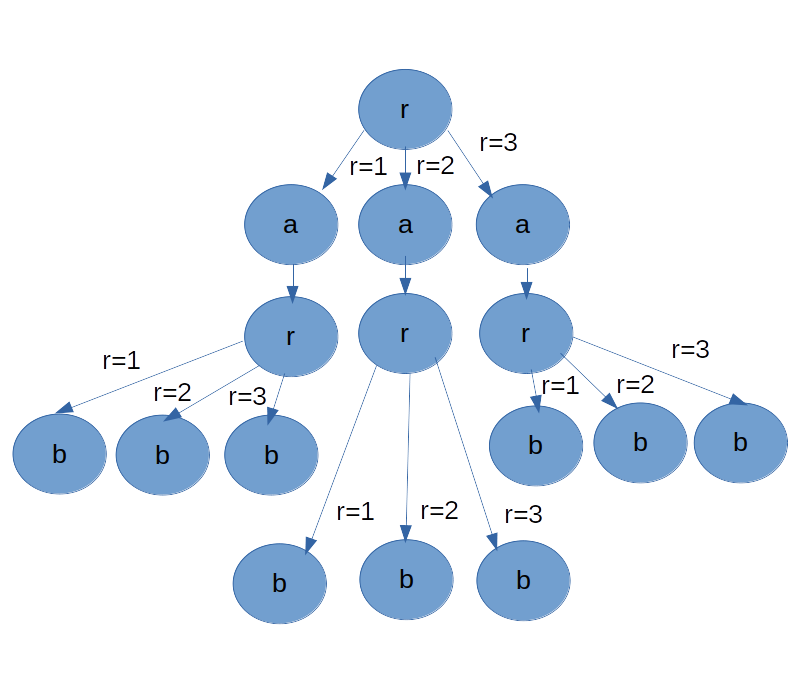
\includegraphics[width=0.9\linewidth]{Graphics/Neigh-Tree}
	\caption{Árbol de vecindad asociado a $rarb$}
	\label{fig:neigh-tree}
\end{figure}

Cada rama del árbol representa un conjunto de soluciones, por tanto, el conjunto de ramas representa una partición de la vecindad a la que está asociado dicho árbol. A los conjuntos hechos por esta partición se les denomina regiones y resultan útiles para encontrar características compartidas en grupos de vecindades. Por ejemplo, es conveniente analizar cuáles son las regiones con mejores soluciones para intensificar en estas la búsqueda de soluciones óptimas.

Luego de generadas las soluciones a partir del Árbol de Vecindad, es necesario conocer sus costos. Para esto se utiliza un Grafo de Evaluación.

\section{Grafo de Evaluación}\label{2-JJ}
Durante la exploración de las vecindades es (generalmente) necesario evaluar las soluciones que se van analizando. Ya sea para retornar inmediatamente una solución mejor a la inicial (estrategia de selección de primera mejora), para devolver la mejor solución (estrategia de selección de mejor vecino) o un vecino aleatorio entre todos los que mejoren la solución (estrategia de selección de mejor vecino aleatorio), en todos los casos hay que determinar el costo de las soluciones exploradas para analizar lo que es "mejor". Encontrar el costo de una solución es lo que se denomina como evaluar.

La evaluación de soluciones es potencialmente costosa. En el caso más simple se debe sumar las distancias entre cada cliente de cada ruta y el depósito. Agregar restricciones implica análisis extra como la aplicación de penalizaciones a rutas con vehículos sobrecargados en el caso de CVRP.

El Grafo de Evaluación, propuesto por Jose Jorge Rodríguez en \ref{2-JJ}, permite evaluar soluciones vecinas a una solución inicial de forma eficiente ya que garantiza que sólo se recalculan los fragmentos de las nuevas soluciones en los que estas se diferencien de la solución inicial.

La estructura propuesta es una representación en forma de grafo de la evaluación de la función objetivo en una determinada solución. Sus nodos están divididos en dos tipos: Nodos de alto nivel y nodos de bajo nivel. Los nodos de bajo nivel representan operaciones (incremento, decremento) que reciben como entradas ciertos nodos de alto nivel y modifican con sus salidas otros nodos de alto nivel.

Por ejemplo, en \ref{fig:eval-graph-1} se muestran los nodos de alto nivel del grafo que representa la solución:

\begin{equation}
s = [(c_1,c_2), (c_3,c_4)]
\end{equation}

Nótese que todas las rutas en el grafo comienzan y terminan con el nodo que representa al depósito. El nodo $cost$ almacena el valor del costo total de la solución.

\begin{figure}
	\centering
	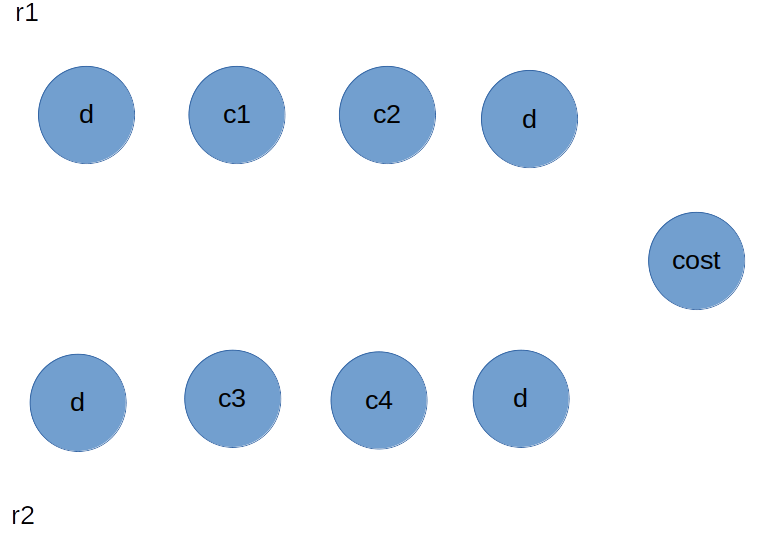
\includegraphics[width=0.9\linewidth]{Graphics/eval-graph-1}
	\caption{Nodos de alto nivel en un grafo de evaluación que representa la solución $s1$ de VRP clásico.}
	\label{fig:eval-graph-1}
\end{figure}

En \ref{fig:eval-graph-2} se muestra una representación del grafo completo para esta solución. Los nodos con símbolo de incremento son nodos de bajo nivel que toman como entrada dos nodos clientes (o depósito) y como salida adicionan al nodo de costo total la distancia entre ellos.

\begin{figure}
	\centering
	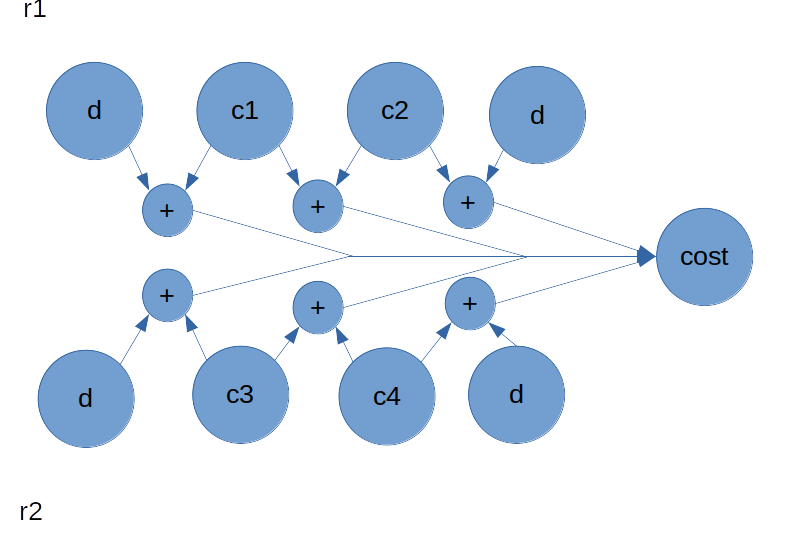
\includegraphics[width=0.9\linewidth]{Graphics/eval-graph-2}
	\caption{Grafo de evaluación que representa la solución $s1$ de VRP clásico.}
	\label{fig:eval-graph-2}
\end{figure}

En \ref{fig:eval-graph-3} se transforma el problema en CVRP utilizando la misma solución. En este caso se agregan los nodos de alto nivel $cap$ que tienen como valor inicial la capacidad del vehículo perteneciente a cada ruta. Los nodos de decremento reciben un cliente como entrada y, como salida, disminuyen la capacidad del vehículo en una cantidad igual a la demanda del cliente. Luego, los nodos $pen$ (también de bajo nivel) reciben como entrada los nodos de capacidad y, en caso de tener estos valor negativo, como salida penalizan el costo total de la solución.

 \begin{figure}
	\centering
	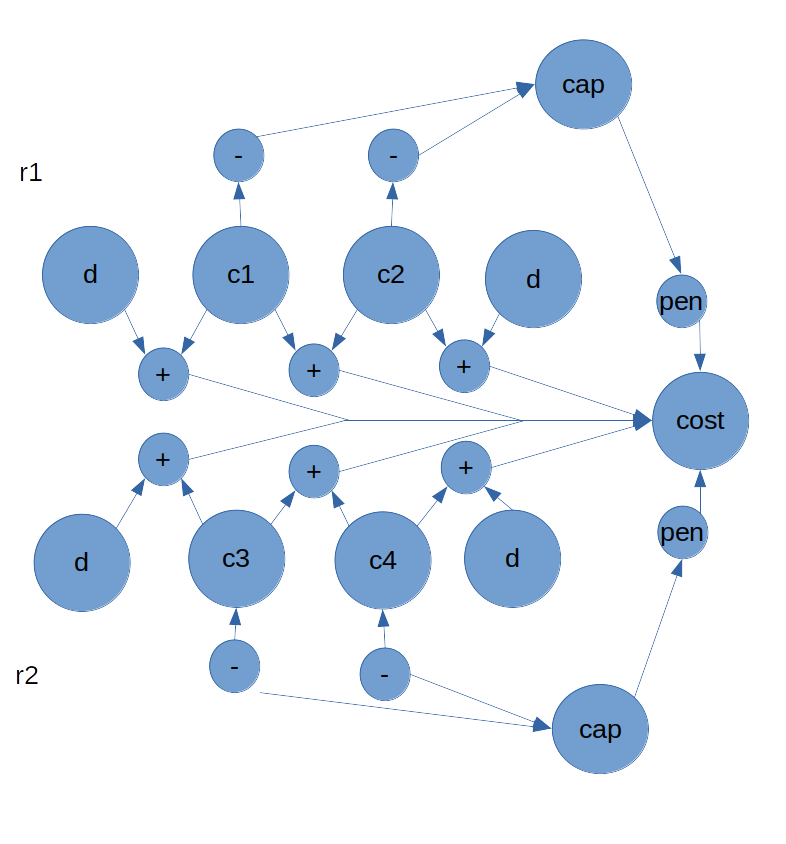
\includegraphics[width=0.9\linewidth]{Graphics/eval-graph-3}
	\caption{Grafo de evaluación que representa la solución $s1$ de VRP con restricciones de capacidad.}
	\label{fig:eval-graph-3}
\end{figure}

Todos los nodos de bajo nivel tienen asociado una función \textbf{evaluate} (para evaluar) y una función \textbf{undo} (para desevaluar) que son ejecutados cuando se agregan o remueven nodos de alto nivel. Por ejemplo, retirar un cliente $C1$ del grafo representado en \ref{fig:eval-graph-2} (VRP clásico) provoca que los dos nodos de incremento que utilizan dicho cliente como entrada se desevalúen y al mismo tiempo se crea un nuevo nodo incremento que recibe como entrada $d$ y $c2$. Luego, insertar a $c1$ al final de la ruta $r2$ implicaría desevaluar el nodo incremento que recibe como entrada a $c4$ y $d$ mientras se crean dos nodos incrementos nuevos, uno recibiendo de entrada a $c4$ y $c1$ mientras que el otro a $c1$ y $d$. El resultado de estas dos operaciones se muestra en \ref{fig:eval-graph-4} y es, precisamente, el grafo resultante de aplicar la siguiente instanciación del criterio $rarb$:

\begin{itemize}
	\item Seleccionar ruta (r1).
	\item Seleccionar cliente (c1) en ruta (r1).
	\item Seleccionar ruta (r2).
	\item Insertar cliente (c1) en posición (3) en ruta (r2).
\end{itemize}

Nótese que luego de aplicar los métodos \textbf{evaluate} y \textbf{undo} correspondientes el nodo $cost$ tiene almacenado el costo de la solución resultante luego de aplicar una instancia del criterio $rarb$. Para encontrar el costo de la nueva solución sólo fue necesario analizar y modificar los nodos en que el grafo de la solución nueva se diferencia con la solución anterior y no todo el grafo. En esto se basa la evaluación "eficiente" del Grafo de Evaluación.

 \begin{figure}
	\centering
	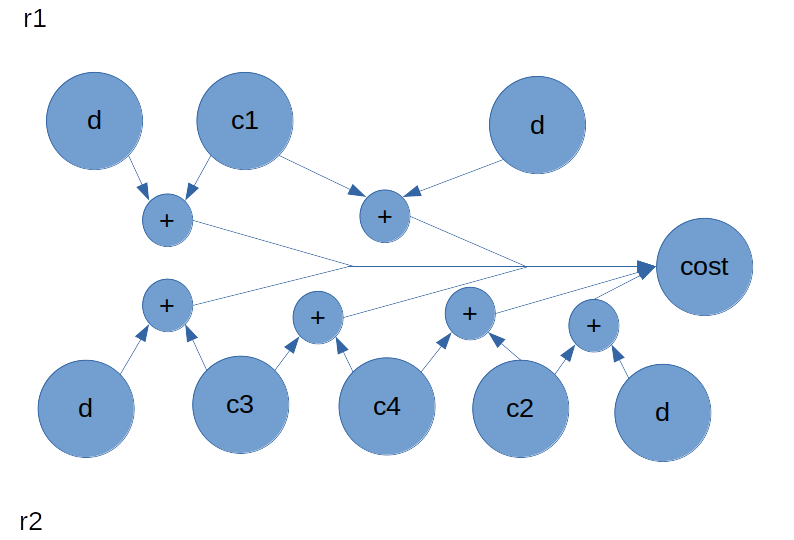
\includegraphics[width=0.9\linewidth]{Graphics/eval-graph-4}
	\caption{Grafo de evaluación que representa la solución $s1$ de VRP clásico luego de aplicada una instancia de $rarb$}
	\label{fig:eval-graph-4}
\end{figure}

Para construir el grafo que representa la solución inicial el usuario debe ingresar el códio de evaluación de esa primera solución. Luego, los costos el resto de las soluciones generadas son obtenidos al aplicar operaciones sobre el grafo inicializado.

Para explorar una vecindad a partir de un criterio es necesario (además de generar y evaluar soluciones) decidir e implementar estrategias de exploración y de selección. A partir de combinaciones de diferentes estrategias se pueden realizar montones de exploraciones distintas.


\section{Combinación de estrategias de exploración y selección.}\label{2-Heidy} 
En el proceso de exploración de una vecindad se parte de una solución inicial, se generan soluciones vecinas a esta (con el Árbol de vecindad) y se evalúan para comparar y obtener mejores soluciones (Grafo de Evaluación). Al explorar, deben también tenerse en cuenta problemas tales como la cardinalidad potencialmente enorme de los vecinos o el retorno de mínimos locales. Para una vecindad muy poblada tal vez dé mejor resultado explorar no todos sus vecinos, sino una porción aleatoria de estos. Tal vez retornar siempre al mejor vecino de cada vecindad pueda provocar el encuentro de un mínimo local que se hubiera evitado seleccionando aleatoriamente cualquier solución que mejorara la inicial.

Al espectro de búsqueda de vecinos en una vecindad se le denomina estrategia de exploración. Algunos ejemplos son:

\begin{itemize}
	\item Exploración exhaustiva: Se analizan todos los vecinos que puedan ser generados.
	\item Exploración aleatoria: Se genera una cantidad fija de vecinos menor que la cardinalidad de la vecindad. La decisión de qué vecinos generar es aleatoria.
\end{itemize}

Además de decidir qué vecinos explorar, también es necesario decidir cuál retornar entre aquellos que mejoran la solución. A esta decisión se le denomina estrategia de selección. Se tiene como ejemplos:

\begin{itemize}
	\item Mejor vecino: Se retorna al mejor vecino entre todos aquellos analizados.
	\item Primera mejora: En el momento en que se encuentra un vecino mejor que el inicial, este es retornado.
	\item Mejora aleatoria: Se retorna un vecino aleatorio entre todos aquellos mejores que la solución inicial.
\end{itemize}

A partir de distintas combinaciones de estrategias de exploración y selección es posible realizar numerosas exploraciones distintas que obtengan diferentes resultados.

La propuesta de Heidy Abreu en \cite{Heidy} permite generar funciones de exploración fabricadas a partir de un criterio, una estrategia de selección y una de exploración. Las estrategias se definen como clases que se pasan como instancias a la función generadora. La función resultante recibe el problema con una solución inicial, ejecuta la exploración y retorna una solución mejor en caso de existir dentro de la vecindad definida por el criterio. En este trabajo, el árbol de vecindad y el grafo de evaluación forman parte también de las funciones de exploración creadas. Un árbol de vecinad genera las soluciones y un grafo de evaluación de usa para evaluarlas. El grafo debe ser pasado como entrada.

La creación automática de funciones de exploración con distintas combinaciones de estrategias de exploración y selección se logra aprovechando sus características comunes y estructuras similares. El código generado en todas las funciones se reparte en cinco regiones que se  unen para generar una función completa. Las regiones y el tipo de código que pertenece a cada una se explicarán en \ref{TODO}.

El trabajo de generación de código y la creación de funciones a partir de estrategias diferentes se facilita mucho gracias a las características del lenguaje Common Lisp.

\section{Common Lisp y sus funcionalidades}\label{2-Lisp}
Common Lisp es un lenguaje de programación multi-paradigma (soporta una combinación de paradigmas de programación tales como la programación imperativa, funcional y orientada a objetos). Facilita el desarrollo de software evolutivo e incremental, con la compilación iterativa de programas eficientes en tiempo de ejecución.

El lenguaje acepta herencia múltiple. Esta característica permite crear jerarquías con clases que implementan funcionalidades de varias clases superiores. Por ejemplo, la clase que representa la estrategia de selección de mejor vecino (\textbf{best-improvement}) hereda de una clase que indica  retorno de mejor solución (\textbf{return-best-solution}) y de otra que indica el uso de un grafo de evaluación (\textbf{use-eval-graph}).

La herencia útil resulta especialmente útil para el presente trabajo cuando se combina con el sistema CLOS (Common Lisp Object System). Un mismo método puede tener numerosas implementaciones (especificaciones) que se ejecutan de acuerdo a los tipos de los parámetros proveídos como entradas. Además, también se ejecutan todas las especificaciones cuyos parámetros coincidan con los ancestros de los tipos de las entradas. Todas las especificaciones se combinan alrededor de un método primario conformando un único método con la unión de todos los códigos. El orden en que se combinan los métodos depende del orden de herencia y de los parámetros :before, :around y :after con que se definen.

Como ejemplo se tiene que para generar el código de la función de exploración para la estrategia de selección de menor vecino se une el código de métodos cuyo parámetro de \text{search-strategy} tenga tipo \textbf{best-improvement}, \textbf{return-best-solution}, \textbf{use-eval-graph} y cualquier otra clase que herede de alguna de estas.




























\chapter{Propuesta de solución}\label{chapter:Solution}

En este capítulo se ofrece la estructura general que representa la solución propuesta para codificar soluciones del VRP a un espacio continuo. Su diseño abstracto mediante dos componentes principales, \textit{encoder} y \textit{decoder}, permite la rápida adaptación de otra arquitectura de redes neuronales al modelo general. 

Como parte de la implementación se formularon dos modelos concretos para resolver el problema de codificación, \textit{\textbf{LinearAEC}} y \textit{\textbf{VAE}}. El primero de ellos está basado en un modelo \textit{autoencoder} clásico y el segundo, en un \textit{variational autoencoder}.

También se describe la etapa de generación y procesamiento de los datos para conformar los conjuntos de entrenamiento, prueba y validación. En este punto se retoman los tipos de representación vectorial de soluciones del VRP expuestos en la sección \ref{2-solS}.

A continuación se explica la idea central del problema, el procesamiento de los datos y el diseño de la solución. 


\section{Definición del problema}

La codificación de soluciones del VRP de un espacio discreto a vectores reales, surge por el interés de investigar el espacio continuo que puede obtenerse con el empleo de un modelo \textit{autoencoders} a partir de soluciones discretas del VRP.
De ahí que sea fundamental lograr una representación continua capaz de capturar sus características y propiedades.

El VRP es un problema de optimización combinatoria cuyo objetivo es minimizar el
 valor de una función de costo $C$ sobre el espacio $\mathcal{S}$ de soluciones, es decir $min \; C(s), \: s\in \mathcal{S}$ teniendo en cuenta las características y restricciones del problema. El espacio $\mathcal{S}$ lo forman soluciones representadas por vectores discretos, bien podrían ser cualquiera de las representaciones vistas en el capítulo \ref{chapter:REV-LL}. En este caso se considera que $\mathcal{S} \subset \mathbb{R}^{n}$, está formado por vectores con la misma estructura que los vectores $p$ analizados en \ref{2-Graph}.
 
 
 %En este caso $\mathcal{S}$ constituye un espacio de soluciones discretas del VRP, bien  y $\mathcal{S} \subset \mathbb{R}^{t}$ para algún $t$.
 
 La intención de este trabajo es obtener una representación $z \in \mathcal{Z}$ a partir de $s$, donde $\mathcal{Z}$ es un espacio continuo $\mathcal{Z} \subset \mathbb{R}^{l}$, para algún $l$. Es decir, determinar una función:
 \begin{equation}
 	f: \mathcal{S} \rightarrow \mathcal{Z},
 \end{equation}
 de forma tal que $f(s) = z$, y además, recuperar la solución codificada en $z$ mediante otra función:
  \begin{equation}
  g: \mathcal{Z} \rightarrow \mathcal{S},
  \end{equation}
 cuyo objetivo es conseguir que el resultado de $g(z) = s'$ sea lo más cercano posible a la entrada original $s$. Con esta idea, las soluciones iniciales $s$ se podrán representar mediante vectores con valores reales cuya dimensión depende de la dimensión del problema, y se conoce como código, vector de contexto o vector latente. 
 
Sea $s$ una solución del VRP, el problema enunciado puede reducirse a aproximar las funciones $f$ y $g$ de forma tal que $f(s) = z$ y $g(z) = s$ con el uso de técnicas de aprendizaje profundo, en particular: modelos \textit{autoencoders}. La funciones $f$ y $g$ se denominan \textit{encoder} y \textit{decoder} respectivamente y están constituidas por redes neuronales. La arquitectura específica del modelo se precisará en la sección \ref{3-GenStruct}, pero antes se describe el proceso seguido para generar los datos empleados en el proceso de entrenamiento.


\section{Procesamiento de datos de entrenamiento}\label{dataProc}

Una cuestión importante que se debe abordar antes de introducir el modelo es el procesamiento y preparación de los datos de entrada tal y como se señaló en \ref{1-etapas}. Como parte de esta etapa, se pueden aplicar varias técnicas que dependen del tipo de datos con los que se cuenta, por ejemplo si son de tipo texto o imagen. 

%En este caso se parte de la generación de soluciones del VRP representadas mediante los vectores $p$ explicados en \ref{2-Graph}, que luego se convierten a matrices 

El procesamiento previo permite una mejor adaptación entre los datos y la red neuronal mediante una serie de técnicas como vectorización de la información y normalización. Considerando que en la representación vectorial expuesta en \ref{2-Graph} con los vectores $p$, los valores no están normalizados, se decidió representar los datos a través de las matrices binarias $M$ analizadas en \ref{2-Matrix}. 

Como el objetivo principal es la codificación de una solución a un vector real, solo interesan en ellas, los clientes y cantidad $m$ de rutas. La conformación del conjunto de datos o soluciones iniciales para una instancia particular con $n$ clientes se desarrolló generando los vectores $p$, que como se había explicado, establecen la adyacencia en el grafo formado a partir de las rutas contenidas en la solución. Una vez obtenido ese conjunto de datos, cada solución del mismo se convierte a la matriz $M$ correspondiente, con el fin de obtener una representación normalizada.   

%Teniendo en cuenta las definiciones \ref{2-pi} y \ref{2-Matrix}, correspondientes a los vectores $p$ y las matrices binarias $M$ respectivamente, la transformación de un vector $p$ a una matriz $M$ se establece como sigue:


%Una instancia de un problema de enrutamiento de vehículos está definida por la cantidad de clientes $n$ y la cantidad de vehículos $m$. La conformación inicial del conjunto de datos para una instancia particular se desarrolló generando vectores $p$ que constituyen planificaciones de $m$ rutas para satisfacer los $n$ clientes. Luego de ello, se realiza una transformación sobre cada vector generado para obtener una  representación normalizada con matrices binarias.

%Sea $s \in \mathcal{S}$ una solución discreta a una instancia del VRP con $n$ clientes y $m$ vehículos, $p$ el vector de dimensión $n$ correspondiente según la interpretación ofrecida con grafos dirigidos, y $M$ la matriz binaria que se obtiene a partir de $p$. Primeramente se retoma la definición de ambas representaciones vectoriales:

%\[p[j]=\left\{
%\begin{array}{rcl}
%i & \mbox{si} & \text{el cliente $j + 1$ va detrás de $i + 1$ en la ruta. }\\
%&
%& \\
%j & \mbox{si} & \text{el cliente $j + 1$ es comienzo de ruta. }  \\
%&
%& \\
%\end{array}
%\right. \]


%\[M[i, j]=\left\{
%\begin{array}{rcl}
%1 & \mbox{si} & \text{el cliente $j + 1$ va detrás de $i + 1$ en la ruta.}\\
%&
%& \\
%1 & \mbox{si} & \text{$i = j$, la ruta está formada por un único cliente i + 1.}  \\
%&
%& \\
%0 & \mbox{eoc}  \\
%\end{array}
%\right. \]


%\[M[i, j]=\left\{
%\begin{array}{rcl}
%\label{Pi2M}
%1 & \mbox{si} & \text{$p[j] = i, \; i \neq j$}\\
%&
%& \\
%1 & \mbox{si} & \text{$p[j] = j, \; j + 1$ es el único cliente en su ruta}  \\
%&
%& \\
%0 & \mbox{eoc}  \\
%\end{array}
%\right. \]

%A continuación se muestra el procedimiento seguido para obtener $M$ a partir de $p$ mediante un ejemplo concreto. En particular se considerá el mismo vector de 9 clientes analizado en \ref{2-Graph}:
%\begin{center}
%	$p = [4, 1, 7, 5, 1, 5, 6, 6, 8],$
%\end{center}
%que se corresponde con la solución a través de listas de rutas:
%\begin{center}
%	$s = [(2, 5, 1), (6, 4), (7, 8, 3), (9)].$
%\end{center}

%Finalmente los pasos realizados se resumen en:
%\begin{eqnarray*}
%	p[0] = 4 \rightarrow  M[4, 0] = 1,\\
%	p[2] = 7 \rightarrow  M[7, 2] = 1,\\
%	p[3] = 5 \rightarrow  M[5, 3] = 1,\\
%	p[4] = 1 \rightarrow  M[1, 4] = 1,\\
%	p[7] = 6 \rightarrow  M[6, 7] = 1,\\
%	p[8] = 8 \rightarrow  M[8, 8] = 1, 
%\end{eqnarray*}

%El resto de las posiciones de $M$ tomarán valor 0 según la tercera condición de \ref{Pi2M}. Finalmente la matriz resultante es:

 %\begin{equation}
%\centering
%\begin{pmatrix}
%0 & 0 & 0 & 0 & 0 & 0 & 0 & 0 & 0\\
%0 & 0 & 0 & 0 & 1 & 0 & 0 & 0 & 0\\
%0 & 0 & 0 & 0 & 0 & 0 & 0 & 0 & 0\\
%0 & 0 & 0 & 0 & 0 & 0 & 0 & 0 & 0\\
%1 & 0 & 0 & 0 & 0 & 0 & 0 & 0 & 0\\
%0 & 0 & 0 & 1 & 0 & 0 & 0 & 0 & 0\\
%0 & 0 & 0 & 0 & 0 & 0 & 0 & 1 & 0\\
%0 & 0 & 1 & 0 & 0 & 0 & 0 & 0 & 0\\
%0 & 0 & 0 & 0 & 0 & 0 & 0 & 0 & 1\\
%\end{pmatrix}
%\end{equation}
%la cual coincide con la misma analizada en \ref{M9}.

%Dada la estructura y propiedades de este tipo de matrices, es fácil revertirlas para obtener la solución $s$ correspondiente. No obstante, como no se establece una biyección entre $s$ y $M$, la generación de los datos será mediante otro array que se nombrará como $pi$. 

Una vez representadas las soluciones del VRP como un vector donde cada componente pertenece al intervalo $[0, 1]$, se puede presentar la estructura general del modelo propuesto en la siguiente sección.

%Como se había mencionado, la solución implementada posee una estructura general a la cual se adaptaron los dos modelos propuestos, específicamente, evidenciada en el uso de sus dos componentes principales. En la siguiente sección se profundiza sobre esta cuestión. 


\section{Estructura general del modelo propuesto}\label{3-GenStruct}

El modelo ofrecido en este trabajo para la codificación de soluciones de un problema VRP, sigue la idea general de los modelos \textit{autoencoders} descritos en \ref{2-AEC} y consiste en dos componentes principales:  \textit{encoder} y \textit{decoder}. En la figura \ref{modelGeneral} se muestra un esquema general del modelo.

\begin{figure}[!h]
	\centering
	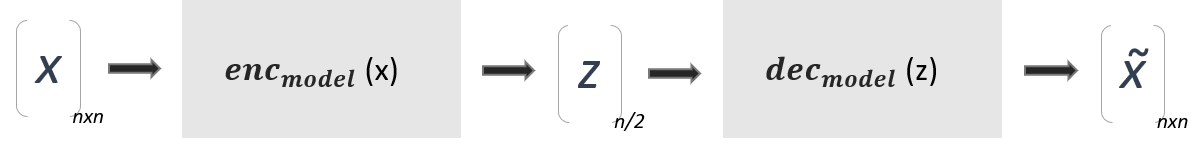
\includegraphics[width=5in]{Graphics/model general.png}
	
	\caption{ \small{Esquema general del modelo propuesto con las componentes \textit{encoder} y \textit{decoder}.}}
	
	\label{modelGeneral}
\end{figure}  

Dichas componentes son las encargadas de aproximar las funciones $f$ y $g$ mencionadas en la definición del problema, de foma tal que $f$ se reemplaza por la componente \textit{encoder} y $g$ se sustituye por la componente \textit{decoder}. Ambas están relacionadas mediante tres vectores que juegan un papel fundamental: el vector de entrada $x$, vector de contexto $z$ y el vector de salida $\tilde{x}$.

Los \textbf{vectores de entrada} constituyen matrices binarias de dimensión $n \times n$ representando a las soluciones del VRP. Además de ser la entrada a la red general, son la entrada de la componente \textit{encoder}. Este devuelve como salida un vector real denotado por $z$ que se conoce como \textbf{vector de contexto}. Posteriormente el \textit{decoder} procesa el vector $z$ y retorna un \textbf{vector de salida} que establece una reconstrucción de la entrada $s$. Tanto la entrada inicial al modelo como la salida final presentan las mismas dimensiones como se observa en el esquema \ref{modelGeneral}.

La configuración de parámetros en las componentes y la dimensión del vector $z$ dependen de la dimensión del problema, por tanto, la arquitectura del modelo se ajusta al tipo de problema particular. Debido a ello es necesario entrenar el modelo para cada dimensión del problema, o sea, para una cantidad de clientes fija.


\subsection{Funcionalidades del modelo propuesto}

La estructura genérica presentada anteriormente permite el uso de las componentes \textit{encoder} y \textit{decoder} de forma independiente, una vez que se entrene el modelo. En este sentido se distinguen tres funcionalidades que cumple el esquema general de la solución.

Siguiendo las definiciones señaladas en este capítulo, se denotará como $s$ el vector de entrada al modelo que representa una solución del VRP, $z$ el vector de contexto representativo de $s$ en el espacio continuo y $s'$ la reconstrucción de $s$ y también salida del modelo. A partir de este momento, las componentes \textit{encoder} y \textit{decoder} también serán tratadas como $enc_{model}$ y $dec_{model}$. 

Las funcionalidades referidas se exponen a continuación:

\begin{itemize}
	\item \textbf{codificar (encode)}: Mediante esta función es posible obtener el vector de código para una entrada $s$ cualquiera, de forma tal que:
	\begin{equation}
		encode(s) = enc_{model}(s) = z
	\end{equation}
	\item \textbf{decodificar (decode)}: A partir de un vector $z$ del espacio continuo, se puede producir la solución correspondiente en el espacio discreto aplicando:
	\begin{equation}
	decode(z) = dec_{model}(z) = s'
	\end{equation}
	
	\item \textbf{predecir (predict)}: Esta función da como resultado el vector reconstruido luego de atravesar por las dos etapas básicas de codificación y decodificación. Su empleo tiene sentido con el modelo ya entrenado para comprobar el desempeño del mismo. El funcionamiento consiste en:
	\begin{equation}
	predict(s) = dec_{model}(enc_{model}(s)) = s'
	\end{equation}
\end{itemize}

En la siguiente sección se profundizará en la descripción de ambos modelos, teniendo en cuenta la arquitectura de redes neuronales seleccionada.


\section{Modelos propuestos}

Como parte de la implementación de la propuesta de solución, se diseñaron dos modelos \textit{autoencoders} para intentar resolver el problema: \textit{\textbf{LinearAEC}} y \textit{\textbf{VAE}}. El primero de ellos conformado sobre la base de un \textit{autoencoders} clásico y el segundo, como su nombre lo indica, ideado a partir de un prototipo de VAE tradicional.

La función de pérdida de reconstrucción empleada en ambos modelos fue $MSE$ (Mean Squared Error), el promedio del cuadrado de las diferencias entre la entrada y la salida. La última capa de cada modelo utiliza la función de activación \textit{sigmoid}, y además, se decidió usar como optimizador \textit{RMSProp}, siguiendo las sugerencias brindadas en \textit{Chollet et al.} \cite{Chollet}. En el resto de las capas de ambos, se utiliza la función de activación \textit{relu}.

En lo adelante se denotarán como $E_i$ y $D_i$ las capas pertenecientes a las redes \textit{encoder} y \textit{decoder} respectivamente. Las características específicas, arquitectura y configuración de ambas propuestas serán abordadas en las siguientes secciones.
 

\subsection{Modelo \textit{LinearAEC}}\label{LinearAEC}

El carácter lineal de esta propuesta está determinado por la arquitectura de capas densas empleado. Tal y como se mencionó en \ref{3-GenStruct}, se encuentra conformado por dos componentes principales y tres vectores importantes. La configuración de la arquitectura y los parámetros correspondientes será detallada a continuación.

\subsubsection{Arquitectura del modelo}

Ambas componentes principales \textit{encoder} y \textit{decoder} constituyen redes neuronales formadas por capas densas. En la figura \ref{AECmodel} se muestra la estructura interna del modelo de inicio a fin:\\

\newpage

\begin{figure}[!h]
\centering
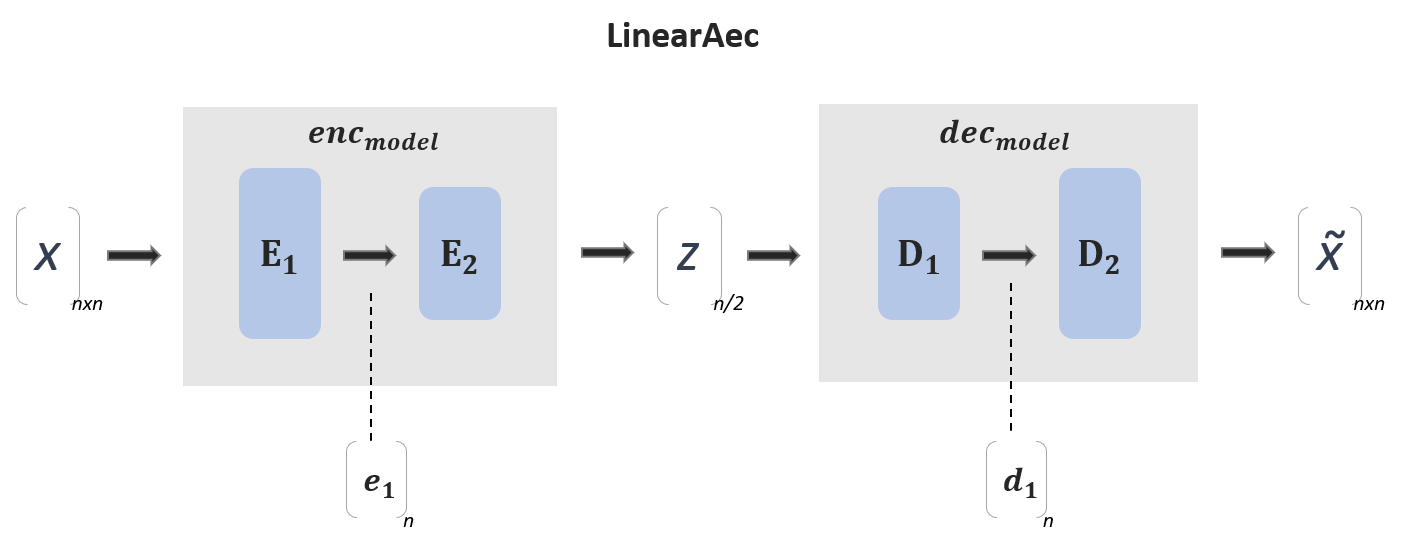
\includegraphics[width=5in]{Graphics/Aecmodel.png}

\caption{ \small{Diagrama del modelo LinearAEC}}

\label{AECmodel}
\end{figure}  


El \textit{encoder} recibe una matriz de entrada $x$ la cual se introduce a la primera capa oculta $E_1$. La salida de esta se conforma mediante la función de activación \textit{relu} y pasa a ser la entrada de la siguiente capa $E_2$, encargada de devolver el vector de contexto $z$. Durante la codificación, la dimensión de los vectores entre una capa y otra va disminuyendo hasta obtener $z$.

Posteriormente, $z$ se convierte en la entrada de la red \textit{decoder} donde será decodificado con el objetivo de recuperar la entrada $x$ inicial. La primera capa de entrada $D_1$ en esta componente, recibe el vector latente y devuelve como salida un vector de mayor dimensión con respecto a $z$, que será la entrada de la última capa $D_2$. Esta capa es la encargada de reconstruir la solución representada en $x$. Durante el proceso de decodificación la dimensión de los vectores de salida va incrementando en correspondencia con la disminución que se establece con la codificación. Por tal motivo, se puede decir que ambos procesos sin simétricos.





\subsection{Modelo \textit{VAE}}
Los VAE constituyen una versión más moderna de los \textit{autoencoders} que proporcionan una noción probabilística para describir un punto del espacio latente. En lugar de generar valores directamente para el estado latente como se hace en \ref{LinearAEC}, el modelo de codificación de un VAE generará parámetros que describen un distribución para cada dimensión en el espacio latente. Dado que se asume una distribución Normal, se generan dos vectores que describen la media y varianza de las distribuciones del espacio. Al generar puntos de tal distribución se obtienen nuevos datos, por eso es considerado un modelo generativo. Finalmente el \textit{decoder} procederá a desarrollar una reconstrucción de la entrada original. 

\subsubsection{Arquitectura del modelo} 


Similar al \textit{LinearAEC}, en el \textit{VAE}, las componentes \textit{encoder} y \textit{decoder} constituyen redes neuronales conformadas por capas densas. Lo interesante y diferente en este modelo, con respecto al \textit{LinearAEC}, es el proceso intermedio donde se genera el vector latente $z$. En la figura \ref{VAEmodel} se muestra un diagrama de la estructura interna del \textit{VAE} implementado, que facilitará la comprensión de sus etapas.\\


\begin{figure}[!h]
	\centering
	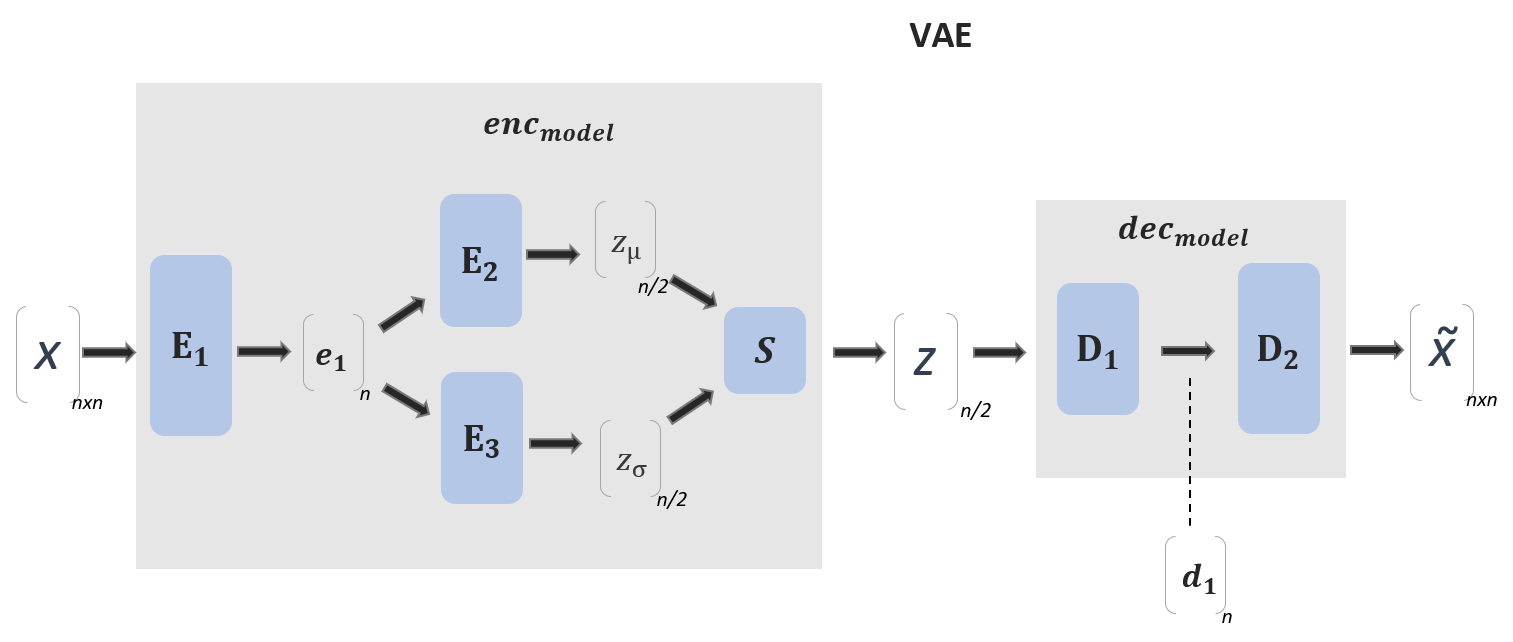
\includegraphics[width=5in]{Graphics/vaemodel.png}
	
	\caption{ \small{Diagrama del modelo VAE}}
	
	\label{VAEmodel}
\end{figure}  

El \textit{encoder} recibe un vector de entrada $x$ de dimensión $nxn$ el cual se procesa por la  capa de entrada $E_1$. A partir de este punto, es donde el proceso de codificación cambia en comparación con el \textit{LinearAEC}. Pues la salida de $E_1$ se introduce paralelamente a otras dos capas ocultas independientes que se identifican como $E_2$ y $E_3$.

El papel de estas nuevas capas es producir los vectores que describen la distribución de las codificaciones $z$. A través de $E_2$ se obtiene $z_{mean}$ y con $E_3$ se origina $z_{log {\_} sigma}$. Hasta el momento se ha explicado el punto número 1 de \ref{VAESteps}, donde se tiene que:

\begin{equation}
	z_{mean} , \; z_{log\_sigma} = enc_{model}(x)
\end{equation} 

Como parte de la generación del vector $z$ con los parámetros de la media y varianza de la distribución, se creó una capa personalizada que se denomina \textit{Sampling}. La capa se denota como $S$ en la figura \ref{VAEmodel}, recibe los parámetros mencionados y su esencia consiste en $	z = z_{mean} + exp(z_{log{\_}sigma})*\epsilon$. 

Una vez generado el vector $z$, este se convierte en la entrada del \textit{decoder}. En lo adelante, el comportamiento del \textit{decoder} es igual a la decodificación en el \text{LinearAEC}. Constituido por dos capas densas consecutivas $D_1$ y $D_2$, donde el vector de salida va aumentando de dimensión de una capa a la otra. Finalmente se obtiene la salida $\tilde{x}$ como reconstrucción de la entrada inicial $x$.\\

En el presente capítulo se expusieron dos modelos concretos para obtener una representación continua de las soluciones del VRP. Ambos se sustentan en la teoría analizada en el capítulo \ref{chapter:REV-LL} e intentan describir una distribución de probabilidad de los vectores de codificación. En el siguiente capítulo se muestran los resultados obtenidos a partir de dos escenarios donde se evalúa el comportamiento de los mismos.



 




\chapter{Experimentos y resultados}\label{chapter:Results}

En este capítulo se presentan los experimentos realizados para evaluar el desempeño de los modelos propuestos: \textit{\textbf{LinearAEC}} y \textit{\textbf{VAE}}.  Se enuncian las métricas empleadas para evaluarlos, así como también la herramienta utilizada para visualizar el espacio latente conformado por los vectores de codificación. Finalmente se muestran los resultados obtenidos en varios ejemplos y se ofrece un análisis a partir de los mismos.

%\section{Generación de los datos}
\section{Consideraciones de la etapa de experimentación}\label{4-Consideraciones}

La generación de un conjunto de soluciones para instancias del VRP con cantidad de clientes considerables, resulta computacionalmente costoso. A ello se le suman los altos requerimientos de cómputo que demanda el proceso de entrenamiento. Por estas razones, se diseñó un marco experimental que fuera factible de ejecutar con recursos limitados.

El equipo de cómputo donde se realizaron los experimentos posee las siguientes propiedades:

\begin{description}
	\item[Memoria:] 16GB - RAM
	\item[Procesador:] \textit{AMD A10-8700P Radeon R6}
	\item[Arquitectura:] \textit{64 bits} 
\end{description}

La implementación de la solución se desarrolló en el lenguaje de programación \textit{Python} y auxiliado del \textit{framework Keras} \cite{keras}. Este último es una biblioteca de código abierto implementada en \textit{Python} y diseñada para posibilitar la experimentación de técnicas de aprendizaje profundo mediante redes neuronales. Sus principales ventajas consisten en ser amigable para el usuario, modular y extensible, de ahí su selección.

Como parte de esta etapa de experimentación, se realizaron varios intentos progresivos de entrenamiento. Se comenzó por conjuntos de datos pequeños hasta finalmente probar con otros de mayor dimensión y así, observar el desempeño con el aumento de los datos. En cada experimento la cantidad de datos destinados para la evaluación del modelo representa el $20\%$ del total, el 80\% restante se conforma de los datos de entrenamiento.

El proceso de aprendizaje pertenece a la categoría de aprendizaje no supervisado debido a que el conjunto de datos está formado por pares de la forma $(M, M)$, donde $M$ constituyen a las matrices binarias de entrada que representan las soluciones del VRP, y a su vez, su respectiva etiqueta o predicción esperada. El objetivo principal evaluado fue la capacidad de generación de soluciones válidas a partir de los vectores de contexto. De esta forma se determina si los vectores codificados son capaces de respresentar de manera continua a las soluciones del problema de enrutamiento.

El entorno de experimentación se desplegó mediante un módulo nombrado \textbf{Evaluador}, que se encarga de iniciar y relacionar la ejecución de los pasos comprendidos en este proceso. El evaluador recibe como argumentos la configuración de los parámetros necesarios para el experimento, el modelo a evaluar (LinearAEC, VAE u otro que cumpla la misma estructura definida en \ref{3-GenStruct}), una función generadora de soluciones del VRP y las métricas empleadas.

Para evaluar los resultados de cada experimento se formularon varias métricas cuantitativas con el fin de comparar la reconstrucción de las soluciones de entrada obtenidas por el \textit{decoder}. Estas se aplican sobre los conjuntos de entrenamiento, validación y prueba que se forman inicialmente con el generador de soluciones. Una vez finalizado el proceso de aprendizaje del modelo particular, se establecen las métricas a partir de una solución de entrada $X$ y su reconstrucción $X_p$:

\subsubsection{Métricas de evaluación}
\begin{description}
	\item[solución válida (valid): ] su valor es 1 si la solución $X_p$ es válida, en otro caso será 0.
	
	\item[mse:] valor del error cuadrático medio entre $X$ y $X_p$.
	
	\item[cantidad de rutas (eqRoutesNumber): ] su valor es 1 si la solución $X_p$ posee la misma cantidad de rutas que la solución $X$, en otro caso será 0.
	
	\item[longitud de rutas (eqRoutesSize): ] su valor es 1 si el conjunto formado por las longitudes de cada ruta en la solución $X$ es igual al conjunto correspondiente para la solución $X_p$, en otro caso será 0.
	
	%\item[inicios de rutas (eqRoutesStarts): ] su valor es 1 si el conjunto formado por los clientes iniciales de cada ruta en la solución $X_p$ es igual al conjunto correspondiente para la solución $X_p$, en otro caso será 0.
	
	%\item[finales de rutas (eqRoutesFinals): ] su valor es 1 si el conjunto formado por los clientes finales de cada ruta en la solución $X_p$ es igual al conjunto correspondiente para la solución $X_p$, en otro caso será 0.
\end{description}

Como se aplican sobre los conjuntos de datos antes mencionados, se calcula el promedio de cada una de ellas en el conjunto completo. 

En la siguiente sección se precisa mejor en qué consiste el experimento general elaborado y se ejemplifica el comportamiento de los modelos implicados con varias configuraciones del experimento.

\subsection{Descripción del marco experimental}

El experimento parte de la creación de una instancia del módulo Evaluador a partir de los argumentos que recibe. La configuración inicial consiste en los siguientes parámetros:
\begin{description}
	\item[\textbf{$n$}:] cantidad de clientes 
	\item[\textbf{$r$}:] cantidad de rutas de las soluciones 
	\item[\textbf{$train$}:] tamaño del conjunto de entrenamiento
	\item[\textbf{$val$}: ] tamaño del conjunto de evaluación
	\item[\textbf{$test$}:] tamaño del conjunto de prueba
	\item[\textbf{$epochs$}:] cantidad de épocas del entrenamiento
\end{description}

También hay que seleccionar el modelo que se evaluará, en ese caso los posibles son las dos propuestas ofrecidas:  \textit{\textbf{LinearAEC}} y \textit{\textbf{VAE}}. Con cada instancia del evaluador se realizará el mismo experimento en ambos modelos para establecer comparaciones con respecto a su rendimiento y capacidad.

La visualización de los datos juega un papel crucial en las aplicaciones de aprendizaje automático, facilitando por lo general, la interpretación y clasificación de los mismos. Por esta razón, se graficó el espacio latente conformado por los vectores reales de codificación mediante una herramienta conocida como \textit{t-SNE}, del inglés \textit{t-distributed stochastic neighbor embedding}. Esta técnica crea una distribución de probabilidad a partir de la distribución gaussiana que define las relaciones entre los puntos en el espacio de alta dimensión, en este caso, el espacio formado por los vectores de contexto denotados por $z$. Además, es capaz de preservar la estructura local y global de los datos.

Con el propósito de evidenciar las consideraciones expuestas en \ref{4-Consideraciones} y la descripción de esta sección, se presentan a continuación una serie de experimentos realizados. Para algunos de ellos, se muestran las funciones de pérdida sobre los datos de entrenamiento y validación, los valores de las métricas definidas y el espacio formado por los puntos de codificación.

\subsection{Ejemplos de experimentos realizados}

\subsubsection{Escenario 1}

La configuración incial del Evaluador se muestra en el cuadro \ref{case1}. Para este escenario el conjunto de datos lo forman soluciones de 25 clientes y 7 rutas 

\begin{table}[h]
	\centering
	\caption{Configuración del experimento en el escenario 1}
	\begin{tabular}{|c|c|c|c|c|c|}
		\hline
		\textbf{n} & \textbf{r} & \textbf{train} & \textbf{val} & \textbf{test} & \textbf{epochs} \\
		\hline
		25 & 7 & 5000 & 1000 & 1000 & 10 \\
		\hline
	\end{tabular}
	\label{case1}
\end{table}

Luego de aplicar las métricas en los conjuntos de entrenamiento, validación y prueba de ambos modelos, se obtienen los resultados resumidos en los cuadros \ref{case1AEC} y \ref{case1VAE}:

\begin{table}[!h]
	\centering
	\caption{Resultado de las métricas en el escenario 1 para el modelo LinearAEC}
	\begin{tabular}{|c|c|c|c|c|}
		\hline
		\textbf{conjunto} & \textbf{ valid} & \textbf{mse} & \textbf{eqRoutesNumber} & \textbf{eqRoutesSize}  \\
		\hline
		\textit{train} & 0.8873 & 0.0264 & 0.0007 & 0.0006 \\
		\hline
		\textit{val} & 0.893 & 0.0268 & 0.002 & 0.0015 \\
		\hline
		\textit{test} & 0.8885 & 0.0268 & 0.0005 & 0.0005 \\
		\hline
		
	\end{tabular}
	\label{case1AEC}
\end{table}

\begin{table}[!h]
	\centering
	\caption{Resultado de las métricas en el escenario 1 para el modelo VAE}
	\begin{tabular}{|c|c|c|c|c|}
		\hline
		\textbf{conjunto} & \textbf{ valid} & \textbf{mse} & \textbf{eqRoutesNumber} & \textbf{eqRoutesSize}  \\
		\hline
		\textit{train} & 0.8803 & 0.0274 & 0.0023 & 0.0021 \\
		\hline
		\textit{val} & 0.87 & 0.0278 & 0.002 & 0.0015 \\
		\hline
		\textit{test} & 0.8765 & 0.0278 & 0.0035 & 0.0025 \\
		\hline
		
	\end{tabular}
	\label{case1VAE}
\end{table}

Los gráficos en \ref{loss_case1} muestran el comportamiento de las funciones de pérdida durante el entrenamiento de ambos modelos.

\begin{figure}[!h]
	\label{loss_case1}
	\subfigure[Pérdida en el modelo LinearAECs]{ 
		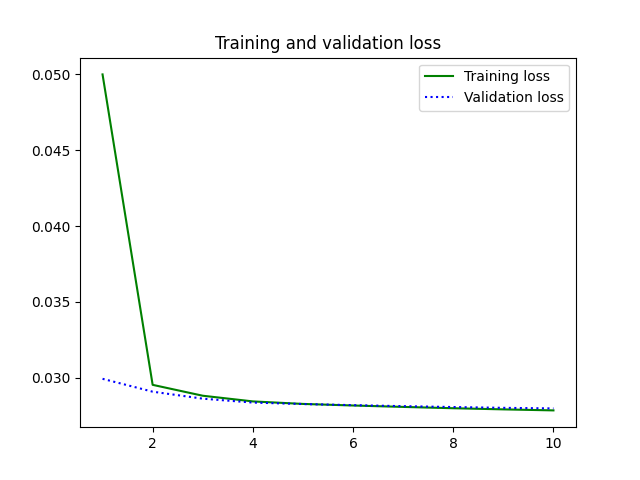
\includegraphics[width=2.9in]{Graphics/experiments/lossFunctions/loss_case1_AEC.png}	
 	}
	\subfigure[Pérdida en el modelo VAE]{ 
		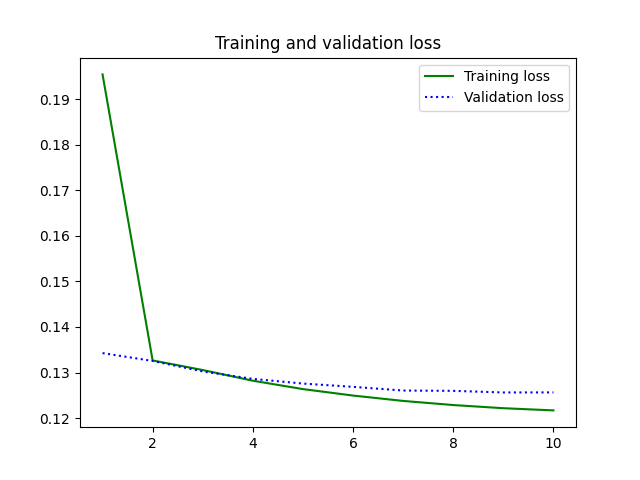
\includegraphics[width=2.9in]{Graphics/experiments/lossFunctions/loss_case1_VAE.png}	
	}
\end{figure}



\begin{figure}[!h]
	\label{space_case1}
	\subfigure[Espacio latente en el conjunto de entrenamiento del modelo LinearAEC]{ 
		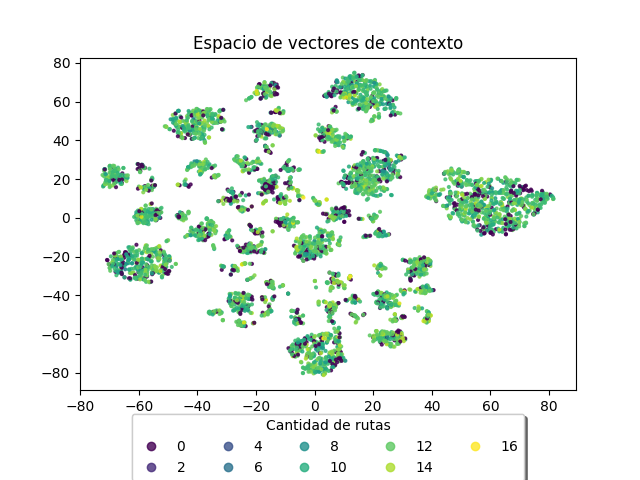
\includegraphics[scale=0.45]{Graphics/experiments/latentSpace/case1_data_AEC.png}	
	}
	\subfigure[Espacio latente en el conjunto de validación del modelo LinearAEC]{ 
		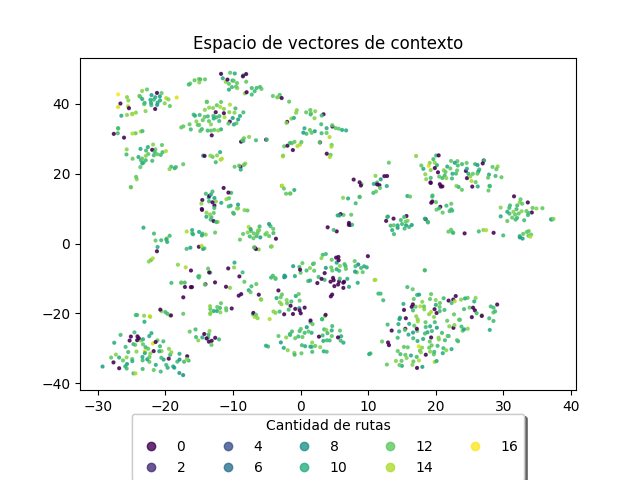
\includegraphics[scale=0.45]{Graphics/experiments/latentSpace/case1_val_AEC.png}	
	}
	%\subfigure[Espacio latente en el conjunto de prueba]{ 
	%	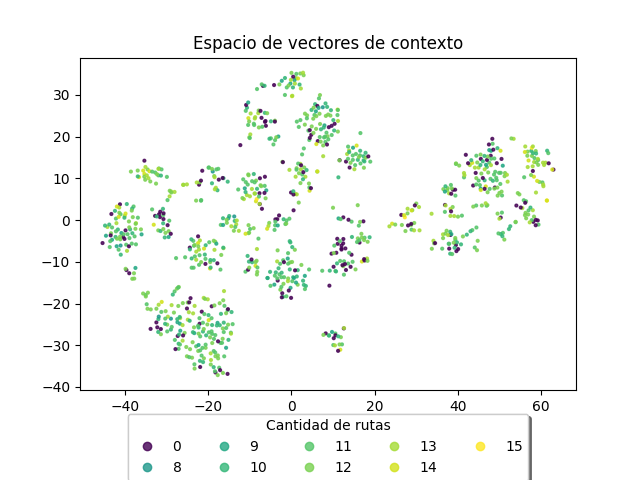
\includegraphics[scale=0.29]{Graphics/experiments/latentSpace/case1_test_AEC.png}	
	%}
\end{figure}

\begin{figure}[!h]
	\label{space_case1vae}
	\subfigure[Espacio latente en el conjunto de entrenamiento del modelo VAE]{ 
		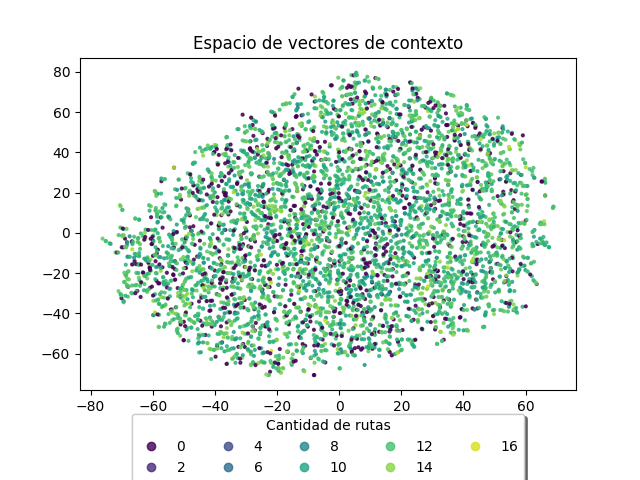
\includegraphics[scale=0.45]{Graphics/experiments/latentSpace/case1_data_VAE.png}	
	}
	\subfigure[Espacio latente en el conjunto de validación del modelo VAE]{ 
		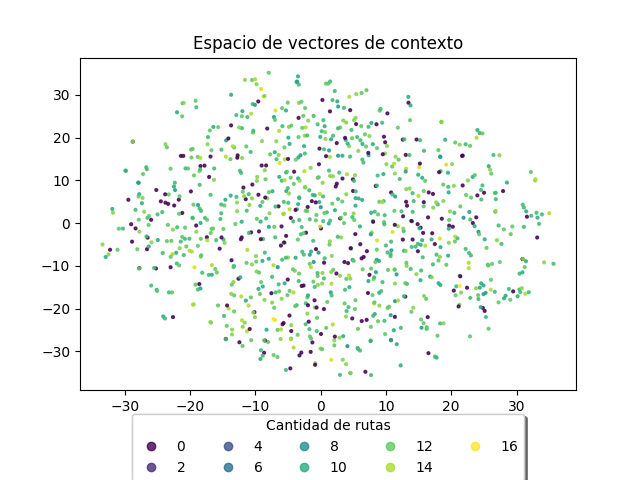
\includegraphics[scale=0.45]{Graphics/experiments/latentSpace/case1_val_VAE.png}	
	}
	%\subfigure[Espacio latente en el conjunto de prueba]{ 
	%	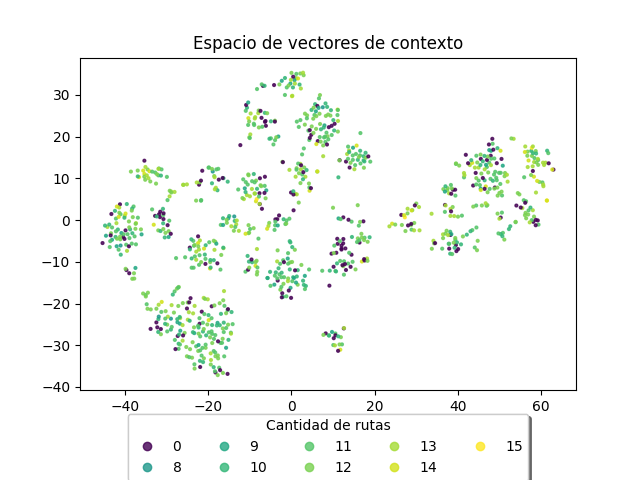
\includegraphics[scale=0.29]{Graphics/experiments/latentSpace/case1_test_AEC.png}	
	%}
\end{figure}

\newpage

\subsubsection{Escenario 2}

La configuración incial del Evaluador se muestra en el cuadro \ref{case2}. Para este escenario el conjunto de datos lo forman soluciones de 20 clientes y 5 rutas 

\begin{table}[h]
	\centering
	\caption{Configuración del experimento en el escenario 2}
	\begin{tabular}{|c|c|c|c|c|c|}
		\hline
		\textbf{n} & \textbf{r} & \textbf{train} & \textbf{val} & \textbf{test} & \textbf{epochs} \\
		\hline
		20 & 5 & 10000 & 2000 & 2000 & 20 \\
		\hline
	\end{tabular}
	\label{case2}
\end{table}

Luego de aplicar las métricas en los conjuntos de entrenamiento, validación y prueba de ambos modelos, se obtienen los resultados resumidos en los cuadros \ref{case2AEC} y \ref{case2VAE}:

\begin{table}[!h]
	\centering
	\caption{Resultado de las métricas en el escenario 2 para el modelo LinearAEC}
	\begin{tabular}{|c|c|c|c|c|}
		\hline
		\textbf{conjunto} & \textbf{ valid} & \textbf{mse} & \textbf{eqRoutesNumber} & \textbf{eqRoutesSize}  \\
		\hline
		\textit{train} & 0.8982 & 0.0342 & 0.0013 & 0.0007 \\
		\hline
		\textit{val} & 0.8745 & 0.0345 & 0.001 & 0.0005 \\
		\hline
		\textit{test} & 0.897 & 0.0346 & 0.0 & 0.0 \\
		\hline
		
	\end{tabular}
	\label{case2AEC}
\end{table}

\begin{table}[!h]
	\centering
	\caption{Resultado de las métricas en el escenario 2 para el modelo VAE}
	\begin{tabular}{|c|c|c|c|c|}
		\hline
		\textbf{conjunto} & \textbf{ valid} & \textbf{mse} & \textbf{eqRoutesNumber} & \textbf{eqRoutesSize}  \\
		\hline
		\textit{train} & 0.8665 & 0.0354 & 0.0319 & 0.0024 \\
		\hline
		\textit{val} & 0.852 & 0.0357 & 0.0245 & 0.002 \\
		\hline
		\textit{test} & 0.874 & 0.0357 & 0.032 & 0.0015 \\
		\hline
		
	\end{tabular}
	\label{case2VAE}
\end{table}

Los gráficos en \ref{loss_case2} muestran el comportamiento de las funciones de pérdida durante el entrenamiento de ambos modelos.

\begin{figure}[!h]
	\label{loss_case2}
	\subfigure[Pérdida en el modelo LinearAECs]{ 
		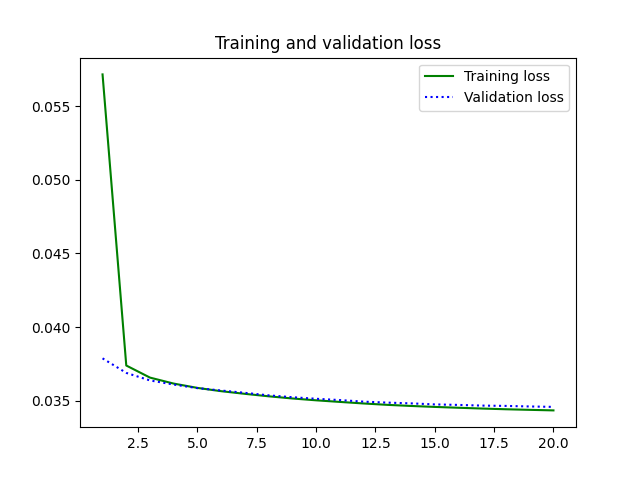
\includegraphics[width=2.9in]{Graphics/experiments/lossFunctions/loss_case2_AEC.png}	
	}
	\subfigure[Pérdida en el modelo VAE]{ 
		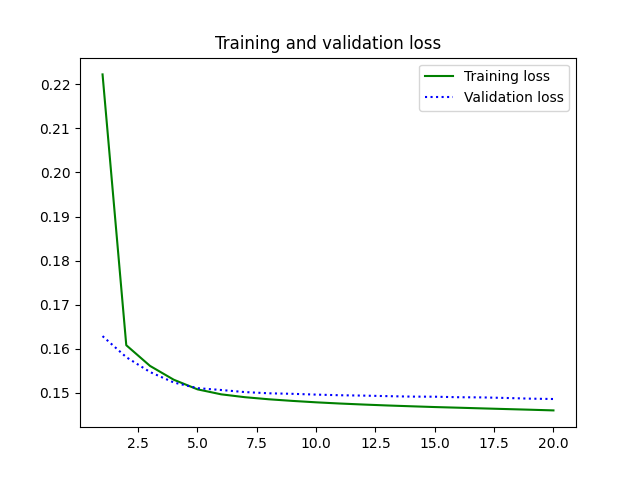
\includegraphics[width=2.9in]{Graphics/experiments/lossFunctions/loss_case2_VAE.png}	
	}
\end{figure}



\begin{figure}[!h]
	\label{space_case2}
	\subfigure[Espacio latente en el conjunto de entrenamiento del modelo LinearAEC]{ 
		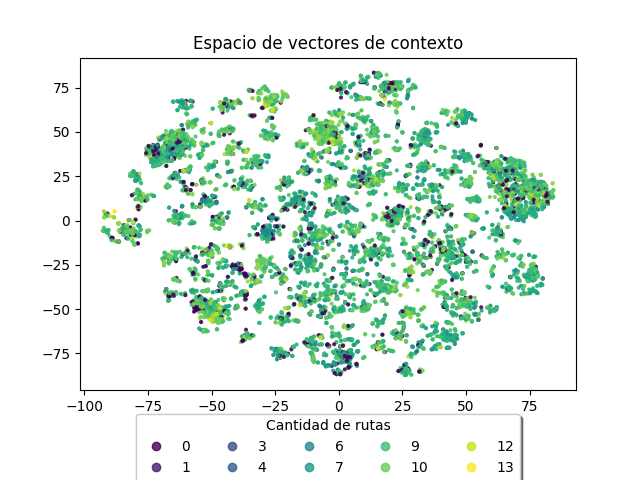
\includegraphics[scale=0.45]{Graphics/experiments/latentSpace/case2_data_AEC.png}	
	}
	\subfigure[Espacio latente en el conjunto de validación del modelo LinearAEC]{ 
		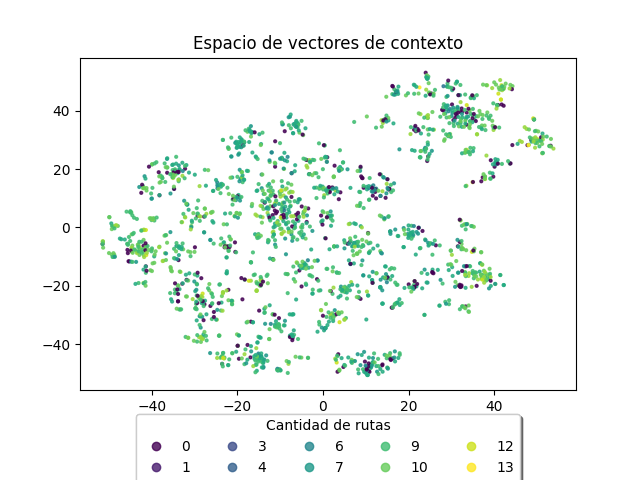
\includegraphics[scale=0.45]{Graphics/experiments/latentSpace/case2_val_AEC.png}	
	}
	%\subfigure[Espacio latente en el conjunto de prueba]{ 
	%	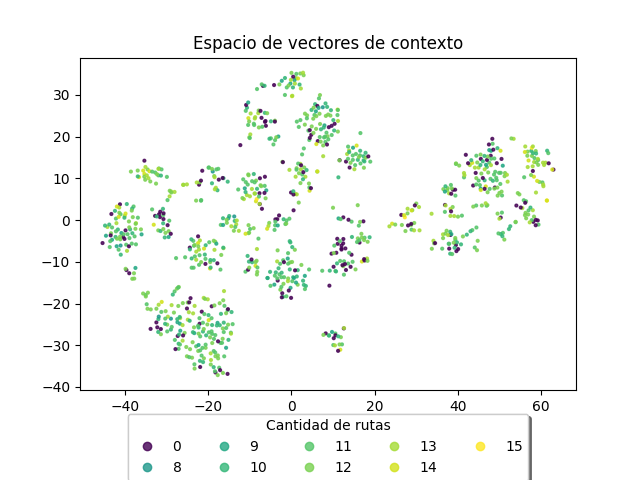
\includegraphics[scale=0.29]{Graphics/experiments/latentSpace/case1_test_AEC.png}	
	%}
\end{figure}

\begin{figure}[!h]
	\label{space_case2vae}
	\subfigure[Espacio latente en el conjunto de entrenamiento del modelo VAE]{ 
		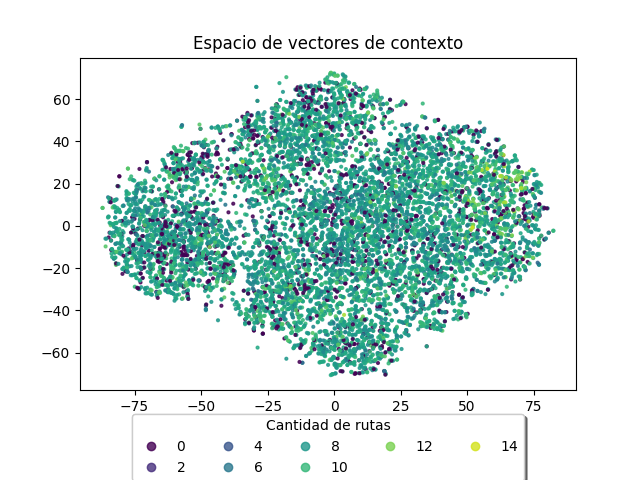
\includegraphics[scale=0.45]{Graphics/experiments/latentSpace/case2_data_VAE.png}	
	}
	\subfigure[Espacio latente en el conjunto de validación del modelo VAE]{ 
		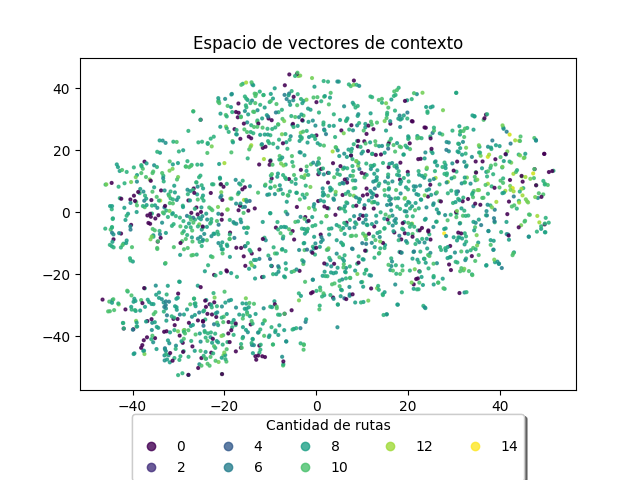
\includegraphics[scale=0.45]{Graphics/experiments/latentSpace/case2_val_VAE.png}	
	}
	%\subfigure[Espacio latente en el conjunto de prueba]{ 
	%	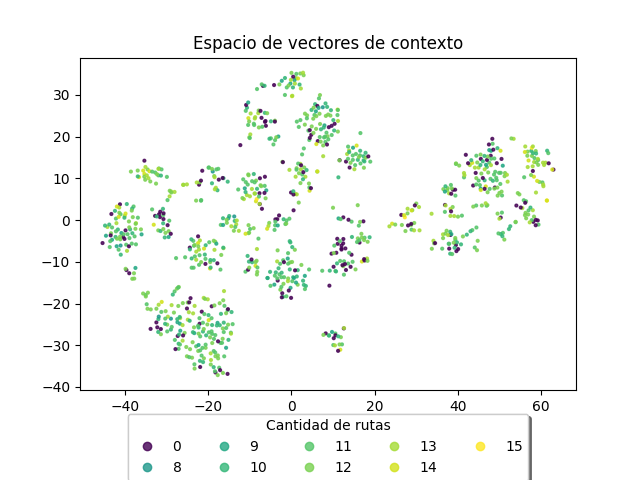
\includegraphics[scale=0.29]{Graphics/experiments/latentSpace/case1_test_AEC.png}	
	%}
\end{figure}

\newpage

\subsection{Análisis de resultados}

Luego de observar los resultados alcanzados en los escenarios anteriores se puede decir que el comportamiento de ambos modelos fue similar en todos los experimentos. Una de las causas es que poseen una arquitectura de capas y configuración de hiperparámetros semejante. 

En los gráficos de las funciones de pérdida se refleja el bajo error característico en los modelos \textit{autoencoders}, con un estilo similar a la pérdida resultante de los trabajos \cite{TrajectoryCompres, VAESparseData}. En el escenario 1, se observa cómo disminuye durante las dos primeras épocas y posteriormente se mantiene moderada.

Un valor de error pequeño no significa en este caso que la reconstrucción alcanzada en la salida se corresponda con la entrada. Este planteamieto se corrobora con los valores de las métricas \textit{eqRoutesNumber} y \textit{eqRoutesSize}, que evalúan la similitud entre una solución de entrada y su salida teniendo en cuenta la cantidad de rutas y las longitudes de cada ruta respectivamente. Pues como se observa en los cuadros \ref{case1AEC}, \ref{case1VAE}, \ref{case2AEC}, \ref{case2VAE}, sus valores son insignificantes y no aportan información sobre el parentezco de las soluciones con respecto a las características que examinan.

 %Debido a la estructura de las matrices $M$, que tienen una cantidad de posiciones igual a $n^2$ y en ellas a lo sumo habrán $n$ posiciones con valor distinto de cero ( $n$ rutas con un cliente distinto en cada una), la diferencia entre la matriz de entrada y la reconstruida a partir de la predicción es pequeña. A partir de esta interpretación, quizás resulte conveniente emplear otra representación vectorial de las soluciones durante el aprendizaje.
 
 A pesar de no alcanzar un nivel adecuado de reconstrucción, en todos los escenarios se comprueba un alto grado de generación de soluciones válidas para una cantidad fija de clientes. La métrica \textit{valid} confirma este efecto. Esta medida arroja en todos los escenarios, y para cada conjunto de datos (\textit{train}, \textit{valid}, \textit{test}), un porciento de generación mayor que $85\%$. Este rendimiento reafirma la capacidad de ambas propuestas como modelos generativos, haciendo posible la generación de nuevas soluciones al explorar el espacio continuo conformado.
 
 Este resultado constituye un logro para este trabajo debido a que se comprueba que las soluciones en el espacio discreto se pueden codificar a un vector real de menor dimensión y que estos, con alta probabilidad se decodifican a una posible solución válida. Se dice posible porque, en este trabajo, no se consideran las restricciones implícitas en el tipo de problema, solo interesa representar una solución a partir de un sistema de rutas.
  
 También se puede apreciar en la visualización de los espacios latentes conformados por las soluciones codificadas, una supremacía de puntos con cantidad de rutas cercana a la cantidad de rutas $r$ de los vectores con los que se entrenaron los modelos. Además, en un mismo modelo se observa que la distribución de puntos en el espacio latente posee una disposición similar. Por ejemplo, para el caso del modelo \textit{LinearAEC} los puntos se organizan formando pequeños conjuntos. A partir de esta interpretación, quizás resulte conveniente explorar ese espacio para descubrir otro tipo de relaciones. Como por ejemplo, determinar si esas agrupaciones están formadas por soluciones con características similares. 
 
 Durante esta etapa de experimentación se prepararon dos escenarios distintos para evaluar el desempeño de ambos modelos. Para ello se calcularon las métricas definidas y se visualizaron los espacios latentes correspondientes. Finalmente se concluye con la obtención de un alto grado de reconstrucción de soluciones válidas.


\backmatter

%===================================================================================
% Chapter: Conclusiones
%===================================================================================
\chapter*{Conclusiones}\label{chapter:conclusions}
\addcontentsline{toc}{chapter}{Conclusiones}
%==================================================================================

%===================================================================================



% Chapter: Recomendaciones
%===================================================================================
\chapter*{Recomendaciones}\label{chapter:recomendaciones}
\addcontentsline{toc}{chapter}{Recomendaciones}
%===================================================================================



\nocite{*}
\bibliographystyle{plain}
\bibliography{Bibliography}


\end{document}